\chapter{Full Development of the amortised calculus}\label{chap:appendix2}

What you find here is an explanation of why the border width keeps flipping from left to right -- which you might have spotted and wondered why that's the case.

Firstly, that is \emph{intended} and thus correct, so there is no reason to worry about this. The reason is that this document is configured as a two-sided book, which means:
\begin{compactitem}
  \item We assume the document will be printed out,
  \item that this will be done in a two-sided mode (i.e., the document will be printed on both sides of each page), and
  \item that the bookbinding will be in the middle, just like in every book.
\end{compactitem}

\begin{wrapfigure}{r}{.55\textwidth}
  \vspace*{-1em}
  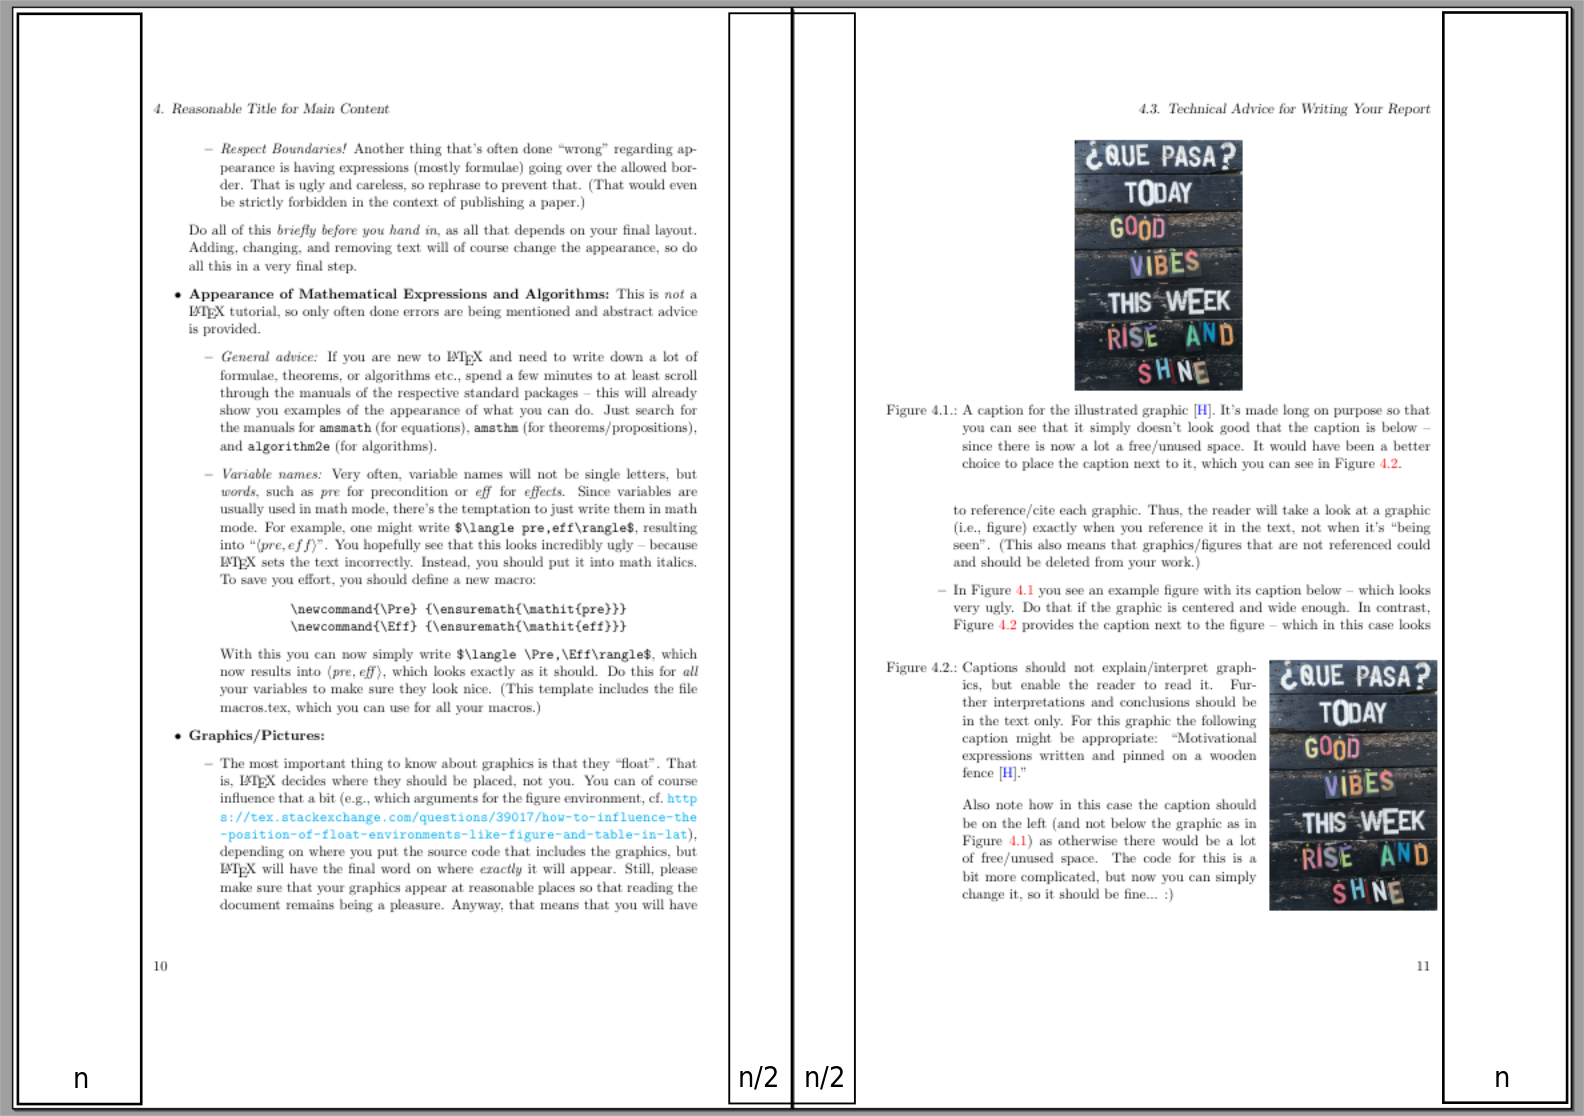
\includegraphics[width=.95\textwidth]{figures/borders--annotated}
  \caption{Illustration showing why page borders flip.\label{fig:pageBorders}}
\end{wrapfigure}

\medskip
When you open the book, there are three borders of equal size~$n$. This however requires that even pages have a border of $n$ on their left and $\frac{n}{2}$ on their right, and odd pages have a border of $\frac{n}{2}$ on their left and $n$ on their right. This is illustrated in Figure~\ref{fig:pageBorders}.

\pagebreak

\section{Formal Definition of $\lambda^{g}_\mathsf{amor}$}
\subsection{Syntax}
\[
\begin{alignedat}{3}
 &\text{Types} &\quad &\tau &\;::={}&
   \alpha\mid\textbf{1}\mid\textbf{b}\mid\tau_1\multimap\tau_2
   \mid\tau_1\otimes\tau_2\mid\tau_1\;\&\;\tau_2\mid\tau_1\oplus\tau_2\\
 &&&&&\mid\mu\alpha.\tau\mid\triangleright\tau\mid\tmonad{I}{\tau}
   \mid L^s\tau\mid\forall\kappa:S.\tau\mid[s]\tau\mid\,!\tau\\[.6ex]
 &\text{Expressions} &&e &\;::={}&\langle\rangle\mid b \mid x \mid \tlam{x}{e}\mid e_1e_2
   \mid\fold e\mid\unfold e\mid e_1\circledast e_2\\
 &&&&&\mid\delay e\mid\ttuple{e_1}{e_2} \mid \tuple{e_1}{e_2}
   \mid\mathsf{fst}\,e\mid\mathsf{snd}\,e\\
 &&&&&\mid\mathsf{inl}\,e\mid\mathsf{inr}\,e\mid \,!e\mid \Lambda.e \mid e\,[\,]\mid nil \mid e_1::e_2\\
 &&&&&\mid(\case{e}{x}{e_1}{y}{e_2})\\
 &&&&&\mid(\lmatch{e}{e_1}{h}{t}{e_2})\\
 &&&&&\mid\lete{!x}{e_1}{e_2}\mid\lete{\ttuple{x}{y}}{e_1}{e_2}\\[.6ex]
 &&&&&\mid\ret e\mid\tick{I}\mid\bind{x}{e_1}{e_2}\mid\pull e\\
 &&&&&\mid\store e\mid\release{x}{e_1}{e_2}\\[.6ex]
 &\text{Indices} &&I,J,s&\;::={}&\kappa\mid N\mid R\mid\clk\mid I+J\mid I-J\\
 &&&&&\mid\textstyle{\sum}_{\kappa<s}I\mid\mathsf{S}^s(I)\\[.6ex]
 &\text{Sorts} &&S &\;::={}&\mathbb N\mid\mathbb R_{\ge0} \\
 &\text{Constraints} &&C &\;::={}&I\leq J\mid I=J\\[.6ex]
 &\text{Affine context} &&\Gamma &\;::={}&\cdot\mid\Gamma,x:\tau\\
 &\text{Unrestricted context} &&\Omega &\;::={}&\cdot\mid\Omega,x:\tau\\
 &\text{Sort context} &&\Theta &\;::={}&\cdot\mid\Theta,\kappa:S\\
 &\text{Constraint context} &&\Delta &\;::={}&\cdot\mid\Delta,C\\
 &\text{Type context} &&\Psi &\;::={}&\cdot\mid\Psi,\alpha
\end{alignedat}
\]

\subsection{Type system}
\begin{figure}[H]
  \centering
  \mprset{sep=1em,andskip=1.5em plus 0.5fil minus 0.5em}
  \renewcommand{\MathparLineskip}{\lineskiplimit=0.6em\lineskip=0.7em plus 0.1em}
  \begin{mathpar}
  \inferrule*[right=S-Var]
      { }
      {\Theta,\kappa:S;\Delta\vdash \kappa:S}

  \inferrule*[right=S-Nat]
      { }
      {\Theta;\Delta\vdash N:\mathbb{N}}

  \inferrule*[right=S-Real]
      { }
      {\Theta;\Delta\vdash R:\mathbb{R}_{\ge0}}
  \\

  \inferrule*[right=S-Clock]
      { }
      {\Theta;\Delta\vdash \clk: \mathbb{N}}

  \inferrule*[right=S-NatReal]
      {\Theta;\Delta\vdash I: \mathbb{N}}
      {\Theta;\Delta\vdash I: \mathbb{R}_{\ge0}}
  \\

  \inferrule*[right=S-Add]
      {\Theta;\Delta\vdash I_1:S \quad \Theta;\Delta\vdash I_2:S}
      {\Theta;\Delta\vdash I_1 + I_2:S}
  \\

  \inferrule*[right=S-Sub]
      {\Theta;\Delta\vdash I:S \quad \Theta;\Delta\vdash J:S
       \quad\Theta;\Delta\models J\leq I}
      {\Theta;\Delta\vdash I-J:S}
  \\

  \inferrule*[right=S-Sum]
      {\Theta;\Delta\vdash J:\mathbb{N} \quad
       \Theta,\kappa:\mathbb{N};\Delta, \kappa < n\vdash I:S \quad
       \Theta;\Delta\models s = \mathsf{S}(s)}
      {\Theta;\Delta\vdash\textstyle{\sum}_{\kappa<s}I:S}
  \\

  \inferrule*[right=S-Shift]
      {\Theta;\Delta\vdash I: S \quad \Theta;\Delta\vdash J:\mathbb{N}
        \quad \Theta;\Delta\models s = \mathsf{S(s)}}
      {\Theta;\Delta\vdash \mathsf{S}^s(I):S}
\end{mathpar} 
  \caption{Sort typing rules for indices}
\end{figure}

\begin{figure}[H]
  \begin{mathpar}
    \inferrule*[right=WF-Var]
      { }
      {\Psi, \alpha;\Theta;\Delta\vdash\alpha}
     
    \inferrule*[right=WF-Unit]
      { }
      {\Psi;\Theta;\Delta\vdash\textbf{1}}
     
    \inferrule*[right=WF-Base]
      { }
      {\Psi;\Theta;\Delta\vdash\textbf{b}}
     
    \inferrule*[right=WF-Arrow]
      {\Psi;\Theta;\Delta\vdash\tau_1 \quad \Psi;\Theta;\Delta\vdash\tau_2 }
      {\Psi;\Theta;\Delta\vdash\tau_1\multimap\tau_2 }
     
    \inferrule*[right=WF-Tensor]
      {\Psi;\Theta;\Delta\vdash\tau_1 \quad \Psi;\Theta;\Delta\vdash\tau_2 }
      {\Psi;\Theta;\Delta\vdash\tau_1\otimes\tau_2 }

    \inferrule*[right=WF-With]
      {\Psi;\Theta;\Delta\vdash\tau_1 \quad \Psi;\Theta;\Delta\vdash\tau_2 }
      {\Psi;\Theta;\Delta\vdash\tau_1\;\&\;\tau_2 }
     
    \inferrule*[right=WF-Sum]
      {\Psi;\Theta;\Delta\vdash\tau_1  \quad \Psi;\Theta;\Delta\vdash\tau_2 }
      {\Psi;\Theta;\Delta\vdash\tau_1\oplus\tau_2 }

    \inferrule*[right=WF-Later]
      {\Psi;\Theta;\Delta\vdash\tau }
      {\Psi;\Theta;\Delta\vdash\triangleright\tau }
     
    \inferrule*[right=WF-Rec]
      {\Psi,\alpha;\Theta;\Delta\vdash\tau 
       \quad \alpha\text{ guarded in }\tau}
      {\Psi;\Theta;\Delta\vdash\mu\alpha.\tau }
     
    \inferrule*[right=WF-Monad]
      {\Psi;\Theta;\Delta\vdash\tau \quad \Theta;\Delta\vdash I: \mathbb{R}_{\ge0}}
      {\Psi;\Theta;\Delta\vdash\tmonad{ I}{\tau} }

    \inferrule*[right=WF-List]
      {\Psi;\Theta;\Delta\vdash\tau\quad\Theta;\Delta\vdash I:\mathbb N
      \quad \Theta;\Delta\models s=\mathsf S(s)}
      {\Psi;\Theta;\Delta\vdash L^s\tau}

    \inferrule*[right=WF-Forall]
      {\Psi;\Theta,\kappa:S;\Delta\vdash\tau}
      {\Psi;\Theta;\Delta\vdash\forall\kappa:S.\tau}

    \inferrule*[right=WF-Pot]
      {\Psi;\Theta;\Delta\vdash\tau \quad 
        \Theta;\Delta\vdash s:\mathbb{R}_{\ge0}
        \quad \Theta;\Delta \models s=\mathsf{S}(s) 
        }
      {\Psi;\Theta;\Delta\vdash[s]\tau}

    \inferrule*[right=WF-Exp]
      {\Psi;\Theta;\Delta\vdash\tau}
      {\Psi;\Theta;\Delta\vdash!\tau}
  \end{mathpar}
  \caption{Type well-formedness}\label{fig:amortized-wf}
\end{figure}

\begin{center}
\fbox{Term Typing judgement: $\hastype{\Theta;\Delta;\Omega;\Gamma}{e}{\tau}$}
\end{center}
\begin{mathparpagebreakable}
\inferrule*[right=T-Var1]
      { }
      {\hastype{\Theta;\Delta;\Omega;\Gamma, x:\tau}{x}{\tau}}

\inferrule*[right=T-Var2]
  { }
  {\hastype{\Theta;\Delta;\Omega,x:\tau;\Gamma}{x}{\tau}}

\inferrule*[right=T-Base]
      { }
      {\hastype{\Theta;\Delta;\Omega;\Gamma}{b}{\textbf{b}}}

\inferrule*[right=T-Unit]
      { }
      {\hastype{\Theta;\Delta;\Omega;\Gamma}{\langle \rangle}{\textbf{1}}}

\inferrule*[right=T-Nil]
      { }
      {\hastype{\Theta;\Delta;\Omega;\Gamma}{nil}{L^0\tau}}

\inferrule*[right=T-Lam]
      {\hastype{\Theta;\Delta;\Omega;\Gamma, x:\tau_1}{e}{\tau_2}}
      {\hastype{\Theta;\Delta;\Omega;\Gamma}{\tlam{x}{e}}{\tau_1 \multimap \tau_2}}

\inferrule*[right=T-App]
      {\hastype{\Theta;\Delta;\Omega;\Gamma_1}{e_1}{\tau_1 \multimap \tau_2}
       \quad \hastype{\Theta;\Delta;\Omega;\Gamma_2}{e_2}{\tau_1}}
      {\hastype{\Theta;\Delta;\Omega;\Gamma_1+\Gamma_2}{e_1e_2}{\tau_2}}

\inferrule*[right=T-TensorI]
      {\hastype{\Theta;\Delta;\Omega;\Gamma_1}{e_1}{\tau_1}
       \quad \hastype{\Theta;\Delta;\Omega;\Gamma_2}{e_2}{\tau_2}}
      {\hastype{\Theta;\Delta;\Omega;\Gamma_1+\Gamma_2}{\ttuple{e_1}{e_2}}{\tau_1\otimes\tau_2}}

\inferrule*[right=T-WithI]
      {\hastype{\Theta;\Delta;\Omega;\Gamma}{e_1}{\tau_1}
       \quad \hastype{\Theta;\Delta;\Omega;\Gamma}{e_2}{\tau_2}}
      {\hastype{\Theta;\Delta;\Omega;\Gamma}{\tuple{e_1}{e_2}}{\tau_1\;\&\;\tau_2}}

\inferrule*[right=T-Fst]
      {\hastype{\Theta;\Delta;\Omega;\Gamma}{e}{\tau_1\;\&\;\tau_2}}
      {\hastype{\Theta;\Delta;\Omega;\Gamma}{\mathsf{fst}\,e}{\tau_1}}

\inferrule*[right=T-Snd]
      {\hastype{\Theta;\Delta;\Omega;\Gamma}{e}{\tau_1\;\&\;\tau_2}}
      {\hastype{\Theta;\Delta;\Omega;\Gamma}{\mathsf{snd}\,e}{\tau_2}}

\inferrule*[right=T-TensorE]
  {\hastype{\Theta;\Delta;\Omega;\Gamma_1}{e_1}{\tau_1\otimes\tau_2}
    \quad\hastype{\Theta;\Delta;\Omega;\Gamma_2,x:\tau_1,y:\tau_2}{e_2}{\tau}}
  {\hastype{\Theta;\Delta;\Omega;\Gamma_1+\Gamma_2}
    {\lete{\ttuple{x}{y}}{e_1}{e_2}}{\tau}}

\inferrule*[right=T-Inl]
      {\hastype{\Theta;\Delta;\Omega;\Gamma}{e}{\tau_1}}
      {\hastype{\Theta;\Delta;\Omega;\Gamma}{\mathsf{inl}\,e}{\tau_1\oplus\tau_2}}

\inferrule*[right=T-Inr]
      {\hastype{\Theta;\Delta;\Omega;\Gamma}{e}{\tau_2}}
      {\hastype{\Theta;\Delta;\Omega;\Gamma}{\mathsf{inr}\,e}{\tau_1\oplus\tau_2}}

\inferrule*[right=T-Prepay]
      {\Theta;\Delta;\Omega;\Gamma\vdash e : \triangleright \tmonad{ I}{\tau}}
      {\hastype{\Theta;\Delta;\Omega;\Gamma}{\pull e}{\tmonad{\mathsf{S}( I)}{\triangleright \tau}}}

\inferrule*[right=T-Cons]
  {
    \hastype{\Theta;\Delta;\Omega;\Gamma_1}{e_1}{\tau}
    \quad \hastype{\Theta;\Delta;\Omega;\Gamma_2}{e_2}{L^s\tau}
    }
  {\hastype{\Theta;\Delta;\Omega;\Gamma_1+\Gamma_2}{e_1::e_2}{L^{s+1}\tau}}

\inferrule*[right=T-Match]
    {\hastype{\Theta;\Delta;\Omega;\Gamma_1}{e}{L^s\tau}
      \\\\ 
      \hastype{\Theta;\Delta,s=0;\Omega;\Gamma_2}{e_1}{\tau'} \quad
      \hastype{\Theta;\Delta,s > 0;\Omega;\Gamma_2,h:\tau,t:L^{s-1}\tau}{e_2}{\tau'}
      }
    {\hastype{\Theta;\Delta;\Omega;\Gamma_1+\Gamma_2}{\lmatch{e}{e_1}{h}{t}{e_2}}{\tau'}}

\inferrule*[right=T-Case]
      {\hastype{\Theta;\Delta;\Omega;\Gamma_1}{e}{\tau_1\oplus\tau_2} \quad
       \hastype{\Theta;\Delta;\Omega;\Gamma_2,x:\tau_1}{e_1}{\tau}
       \quad \hastype{\Theta;\Delta;\Omega;\Gamma_2,y:\tau_2}{e_2}{\tau}}
      {\hastype{\Theta;\Delta;\Omega;\Gamma_1+\Gamma_2} {\case{e}{x}{e_1}{y}{e_2}}{\tau}}

\inferrule*[right=T-Iabs]
      {\hastype{\Theta,\kappa:S;\Delta;\Omega;\Gamma}{e}{\tau}}
      {\hastype{\Theta;\Delta;\Omega;\Gamma}{\Lambda.e}{\forall\kappa:S.\tau}}

\inferrule*[right=T-Iapp]
      {\hastype{\Theta;\Delta;\Omega;\Gamma}{e}{\forall\kappa:S.\tau}
       \quad \Theta;\Delta\vdash I:S}
      {\hastype{\Theta;\Delta;\Omega;\Gamma}{e\,[\,]}{\tau[I/\kappa]}}

\inferrule*[right=T-Sub]
      {\hastype{\Theta;\Delta;\Omega;\Gamma}{e}{\tau}
       \quad \Theta;\Delta\vdash\tau <: \tau'}
      {\hastype{\Theta;\Delta;\Omega;\Gamma}{e}{\tau'}}

\inferrule*[right=T-Weaken]
      {\hastype{\Theta;\Delta;\Omega;\Gamma}{e}{\tau}
       \\\\ \Theta;\Delta\vdash\Omega'<:\Omega
       \quad\Theta;\Delta\vdash\Gamma'<:\Gamma}
      {\hastype{\Theta;\Delta;\Omega';\Gamma'}{e}{\tau}}

\inferrule*[right=T-Fold]
      {\hastype{\Theta;\Delta;\Omega;\Gamma}{e}{\tau[\mu\alpha.\tau/\alpha]}}
      {\hastype{\Theta;\Delta;\Omega;\Gamma}{\fold e}{\mu\alpha.\tau}}

\inferrule*[right=T-Unfold]
      {\hastype{\Theta;\Delta;\Omega;\Gamma}{e}{\mu\alpha.\tau}}
      {\hastype{\Theta;\Delta;\Omega;\Gamma}{\unfold e}{\tau[\mu\alpha.\tau/\alpha]}}

\inferrule*[right=T-Next]
      {\hastype{\Theta;\Delta;\Omega;\Gamma}{e}{\tau}}
      {\hastype{\Theta;\Delta;\Omega;\Gamma}{\delay e}{\triangleright \tau}}

\inferrule*[right=T-Napp]
      {\hastype{\Theta;\Delta;\Omega;\Gamma_1}{e_1}{\triangleright (\tau_1 \multimap \tau_2)}
       \quad \hastype{\Theta;\Delta;\Omega;\Gamma_2}{e_2}{\triangleright \tau_1}}
      {\hastype{\Theta;\Delta;\Omega;\Gamma_1+\Gamma_2}{e_1 \circledast e_2}{\triangleright \tau_2}}

\inferrule*[right=T-Ret]
      {\hastype{\Theta;\Delta;\Omega;\Gamma}{e}{\tau}}
      {\hastype{\Theta;\Delta;\Omega;\Gamma}{\ret e}{\tmonad{0}{\tau}}}

\inferrule*[right=T-Tick]
      {\Theta;\Delta\vdash I:\mathbb{R}_{\ge0}}
      {\hastype{\Theta;\Delta;\Omega;\Gamma}{\,\tick{ I}}{\tmonad{ I}{\textbf{1}}}}

\inferrule*[right=T-Bind]
      {\hastype{\Theta;\Delta;\Omega;\Gamma_1}{e_1}{\tmonad{ I_1}{\tau_1}}
       \quad \hastype{\Theta;\Delta;\Omega;\Gamma_2,x:\tau_1}{e_2}{\tmonad{ I_2}{\tau_2}}}
      {\hastype{\Theta;\Delta;\Omega;\Gamma_1+\Gamma_2}{\bind{x}{e_1}{e_2}}{\tmonad{( I_1 + I_2)}{\tau_2}}}

\inferrule*[right=T-ExpI]
  {\hastype{\Theta;\Delta;\Omega;\cdot}{e}{\tau}}
  {\hastype{\Theta;\Delta;\Omega;\cdot}{!e}{!\tau}}

\inferrule*[right=T-ExpE]
  {\hastype{\Theta;\Delta;\Omega;\Gamma_1}{e_1}{!\tau_1}
    \quad\hastype{\Theta;\Delta;\Omega,x:\tau_1;\Gamma_2}{e_2}{\tau_2}}
  {\hastype{\Theta;\Delta;\Omega;\Gamma_1+\Gamma_2}
    {\lete{!x}{e_1}{e_2}}{\tau_2}}

\inferrule*[right=T-Store]
  {\hastype{\Theta;\Delta;\Omega;\Gamma}{e}{\tau}
    \quad\Theta;\Delta\vdash s:\mathbb{R}_{\ge0}}
  {\hastype{\Theta;\Delta;\Omega;\Gamma}{\store e}{\tmonad{s}{([s]\tau)}}}

\inferrule*[right=T-Release]
  {\hastype{\Theta;\Delta;\Omega;\Gamma_1}{e_1}{[s]\tau_1}
    \quad\hastype{\Theta;\Delta;\Omega;\Gamma_2,x:\tau_1}{e_2}
      {\tmonad{(s+I)}{\tau_2}}}
  {\hastype{\Theta;\Delta;\Omega;\Gamma_1+\Gamma_2}
    {\release{x}{e_1}{e_2}}{\tmonad{I}{\tau_2}}}

\end{mathparpagebreakable}
\captionof{figure}{Term typing judgement}

\begin{figure}[H]
  \begin{mathpar}
    \inferrule*[right=Sub-Monad]
      {\Theta;\Delta\vdash \tau <: \tau' \quad \Theta;\Delta\models I\leq I'}
      {\Theta;\Delta\vdash \tmonad{I}{\tau} <: \tmonad{ I'}{\tau'}}

    \inferrule*[right=Sub-Refl]
      { }
      {\Theta;\Delta\vdash \tau <: \tau}

    \inferrule*[right=Sub-Trans]
      {\Theta;\Delta\vdash \tau_1 <: \tau_2 \quad \Theta;\Delta\vdash \tau_2 <: \tau_3}
      {\Theta;\Delta\vdash\tau_1 <: \tau_3}

    \inferrule*[right=Sub-Arrow]
      {\Theta;\Delta\vdash \tau_1' <: \tau_1 \quad \Theta;\Delta\vdash \tau_2 <: \tau_2'}
      {\Theta;\Delta\vdash \tau_1 \multimap \tau_2 <: \tau_1' \multimap \tau_2'}

    \inferrule*[right=Sub-Tensor]
      {\Theta;\Delta\vdash \tau_1 <: \tau_1' \quad \Theta;\Delta\vdash \tau_2 <: \tau_2'}
      {\Theta;\Delta\vdash \tau_1 \otimes \tau_2 <:  \tau_1' \otimes \tau_2'}

    \inferrule*[right=Sub-With]
      {\Theta;\Delta\vdash \tau_1 <: \tau_1' \quad \Theta;\Delta\vdash \tau_2 <: \tau_2'}
      {\Theta;\Delta\vdash \tau_1\;\&\;\tau_2 <: \tau_1'\;\&\; \tau_2'}

    \inferrule*[right=Sub-Sum]
      {\Theta;\Delta\vdash \tau_1 <: \tau_1' \quad \Theta;\Delta\vdash \tau_2 <: \tau_2'}
      {\Theta;\Delta\vdash \tau_1 \oplus \tau_2 <:  \tau_1' \oplus \tau_2'}

    \inferrule*[right=Sub-List]
      {\Theta;\Delta\vdash \tau <: \tau'}
      {\Theta;\Delta\vdash L^s\tau <: L^s\tau'}

    \inferrule*[right=Sub-IndexPoly]
      {\Theta,\kappa:S;\Delta\vdash\tau<:\tau'}
      {\Theta;\Delta\vdash
        \forall\kappa:S.\tau<:\forall\kappa:S.\tau'}

    \inferrule*[right=Sub-Later]
      {\Theta;\Delta\vdash \tau <:  \tau'}
      {\Theta;\Delta\vdash \triangleright \tau <: \triangleright \tau'}

    \inferrule*[right=Sub-Rec]
      {\Theta;\Delta\vdash \tau <: \tau'}
      {\Theta;\Delta\vdash \mu\alpha.\tau <: \mu\alpha.\tau'}

    \inferrule*[right=Sub-Pot]
      {\Theta;\Delta\vdash\tau<:\tau'\quad\Theta;\Delta\models s'\leq s}
      {\Theta;\Delta\vdash[s]\tau<:[s']\tau'}

    \inferrule*[right=Sub-Exp]
      {\Theta;\Delta\vdash\tau<:\tau'}
      {\Theta;\Delta\vdash!\tau<:!\tau'}

 \inferrule*[right=Sub-Abase]
  { }
  {\Theta;\Delta\vdash\Gamma<:\cdot}

 \inferrule*[right=Sub-Aind]
  {x:\tau'\in\Gamma_1\quad\Theta;\Delta\vdash\tau'<:\tau
    \quad \Theta;\Delta\vdash\Gamma_1/x<:\Gamma_2}
  {\Theta;\Delta\vdash\Gamma_1<:\Gamma_2,x:\tau}

 \inferrule*[right=Sub-Ubase]
  { }
  {\Theta;\Delta\vdash\Omega<:\cdot}

 \inferrule*[right=Sub-Uind]
  {x:\tau'\in\Omega_1\quad\Theta;\Delta\vdash\tau'<:\tau 
    \quad \Theta;\Delta\vdash\Omega_1/x<:\Omega_2}
  {\Theta;\Delta\vdash\Omega_1<:\Omega_2,x:\tau}
\end{mathpar}
\caption{Subtyping judgement}
\end{figure}

\subsection{Semantics}
\begin{figure}[H]
  \centering
  \fbox{Values: $\isval{e}{n}$}
  \begin{mathpar}
    \inferrule*[right=V-Constant]
      { e \in 
        \{\langle\rangle, b, x, \tlam{x}{e}, nil, 
          \Lambda.e, \ret e, \tick{I}, \bind{x}{e_1}{e_2},\pull e,\store e, \release{x}{e_1}{e_2}\}
      }
      {\isval{e}{n}}

    \inferrule*[right=V-Cons]
      {\isval{e_1}{n}\quad\isval{e_2}{n}}
      {\isval{e_1::e_2}{n}}

    \inferrule*[right=V-Tensor]
      {\isval{e_1}{n}\quad\isval{e_2}{n}}
      {\isval{\ttuple{e_1}{e_2}}{n}}

    \inferrule*[right=V-With]
      {\isval{e_1}{n}\quad\isval{e_2}{n}}
      {\isval{\tuple{e_1}{e_2}}{n}}

    \inferrule*[right=V-Inl]
      {\isval{e}{n}}
      {\isval{\mathsf{inl}\,e}{n}}

    \inferrule*[right=V-Inr]
      {\isval{e}{n}}
      {\isval{\mathsf{inr}\,e}{n}}

    \inferrule*[right=V-Exp]
      {\isval{e}{n}}
      {\isval{!e}{n}}

    \inferrule*[right=V-Fold]
      {\isval{e}{n}}
      {\isval{\fold e}{n}}

    \inferrule*[right=V-NextBase]
      { }
      {\isval{\delay e}{0}}

    \inferrule*[right=V-NextInd]
      {\isval{e}{n}}
      {\isval{\delay e}{n+1}}
  \end{mathpar}
  \caption{Value judgement}
  \label{fig:amortized-values}
\end{figure}

\begin{figure}[H]
  \centering
  \begin{mathpar}[\mprset{andskip=1.5em,lineskip=6pt}]

    \inferrule*[right=E-App]
      {e[v_2/x]\Downarrow_n v \quad 
       e_1\Downarrow_n\tlam{x}{e}\quad e_2\Downarrow_n v_2}
      {e_1e_2\Downarrow_n v}

    \inferrule*[right=E-Add]
      {e_1\Downarrow_n\overline{k_1}\quad
       e_2\Downarrow_n\overline{k_2}}
      {e_1+e_2\Downarrow_n\overline{k_1+k_2}}

    \inferrule*[right=E-TensorI]
      {e_1\Downarrow_n v_1\quad e_2\Downarrow_n v_2}
      {\ttuple{e_1}{e_2}\Downarrow_n\ttuple{v_1}{v_2}}

    \inferrule*[right=E-TensorE]
      {e_1\Downarrow_n\ttuple{v_1}{v_2}\quad
       e_2[v_1/x,v_2/y]\Downarrow_n v}
      {\lete{\ttuple{x}{y}}{e_1}{e_2}\Downarrow_n v}

    \inferrule*[right=E-WithI]
      {e_1\Downarrow_n v_1\quad e_2\Downarrow_n v_2}
      {\tuple{e_1}{e_2}\Downarrow_n \tuple{v_1}{v_2}}

    \inferrule*[right=E-Fst]
      {e\Downarrow_n\tuple{v_1}{v_2}}
      {\mathsf{fst}\,e\Downarrow_n v_1}

    \inferrule*[right=E-Snd]
      {e\Downarrow_n\tuple{v_1}{v_2}}
      {\mathsf{snd}\,e\Downarrow_n v_2}

    \inferrule*[right=E-Inl]
      {e\Downarrow_n v}
      {\mathsf{inl}\,e\Downarrow_n\mathsf{inl}\,v}

    \inferrule*[right=E-Inr]
      {e\Downarrow_n v}
      {\mathsf{inr}\,e\Downarrow_n\mathsf{inr}\,v}
    \\

    \inferrule*[right=E-CaseL]
      {e\Downarrow_n\mathsf{inl}\,v\quad
       e_1[v/x]\Downarrow_n v'}
      {\case{e}{x}{e_1}{y}{e_2}\Downarrow_n v'}

    \inferrule*[right=E-CaseR]
      {e\Downarrow_n\mathsf{inr}\,v\quad
       e_2[v/y]\Downarrow_n v'}
      {\case{e}{x}{e_1}{y}{e_2}\Downarrow_n v'}

    \\

    \inferrule*[right=E-Cons]
      {e_1\Downarrow_n v\quad e_2\Downarrow_n l}
      {e_1::e_2\Downarrow_n v::l}

    \inferrule*[right=E-MatchNil]
      {e\Downarrow_n nil\quad e_1\Downarrow_n v}
      {\lmatch{e}{e_1}{h}{t}{e_2}\Downarrow_n v}

    \inferrule*[right=E-MatchCons]
      {e\Downarrow_n v_h::l\quad
       e_2[v_h/h][l/t]\Downarrow_n v}
      {\lmatch{e}{e_1}{h}{t}{e_2}\Downarrow_n v}
      
    \\

    \inferrule*[right=E-NappBase]
      {e_1\Downarrow_0\delay e_1'\quad
       e_2\Downarrow_0\delay e_2'}
      {e_1\circledast e_2\Downarrow_0\delay(e_1'e_2')}

    \inferrule*[right=E-NappInd]
      {e[v_2/x]\Downarrow_n v \quad 
       e_1\Downarrow_{n+1}\delay(\lambda x.e)\quad
       e_2\Downarrow_{n+1}\delay v_2}
      {e_1\circledast e_2\Downarrow_{n+1}\delay v}
    \\
    \inferrule*[right=E-NextBase]
      { }
      {\delay e\Downarrow_0\delay e}

    \inferrule*[right=E-NextInd]
      {e\Downarrow_n v}
      {\delay e\Downarrow_{n+1}\delay v}

    \inferrule*[right=E-Fold]
      {e\Downarrow_n v}
      {\fold e\Downarrow_n\fold v}

    \inferrule*[right=E-Unfold]
      {e\Downarrow_n\fold v}
      {\unfold e\Downarrow_n v}

    \inferrule*[right=E-Iapp]
      {e\Downarrow_n\Lambda.e'\quad
       e' \Downarrow_n v}
      {e\,[\,]\Downarrow_n v}

    \inferrule*[right=E-ExpI]
      {e \Downarrow_n v}
      {!e \Downarrow_n !v}

    \inferrule*[right=E-ExpE]
      {e_1\Downarrow_n !v\quad e_2[v/x]\Downarrow_n v}
      {\lete{!x}{e_1}{e_2}\Downarrow_n v}

    \inferrule*[right=E-Val]
      {\isval{v}{n}}
      {v\Downarrow_n v}
    \end{mathpar}
  \caption{Pure Evaluation judgement}
\end{figure}

\begin{figure}[H]
  \centering
  \begin{mathpar}[\mprset{andskip=1.5em,lineskip=6pt}]

    \inferrule*[right=E-Return]
      {e\Downarrow_n v}
      {\ret e\Downarrow_{n,i}^{0}v}

    \inferrule*[right=E-Tick]
      { }
      {\tick{I}\Downarrow_{n,i}^{I(i)}\langle\rangle}

    \inferrule*[right=E-Bind]
      {
       e_1\Downarrow_n v_1\quad
       v_1\Downarrow_{n,i}^{c_1}v_1'\quad
       e_2[v_1'/x]\Downarrow_n v_2  \quad
       v_2\Downarrow_{n,i}^{c_2}v_2'}
      {\bind{x}{e_1}{e_2}\Downarrow_{n,i}^{c_1+c_2}v_2'}

    \inferrule*[right=E-Prepay]
      {e\Downarrow_{n+1}\delay v\quad
       v\Downarrow_{n,i+1}^{c}v'}
      {\pull e\Downarrow_{n+1,i}^{c}\delay v'}

    \inferrule*[right=E-Store]
      {e\Downarrow_n v}
      {\store e\Downarrow_{n,i}^{0}v}

  \inferrule*[right=E-Release]
    { e_1\Downarrow_n v_1 \quad
      e_2[v_1/x]\Downarrow_n v_2 
      \quad v_2\Downarrow_{n,i}^{c}v}
    {\release{x}{e_1}{e_2}\Downarrow_{n,i}^{c}v}
    \end{mathpar}
  \caption{Forcing Evaluation judgement}
\end{figure}

\begin{appbdef}[Type size]
\begin{align*}
  &|\alpha|=|\textbf{b}|=|\textbf{1}|=|\triangleright\tau|=1, \\
  &|\tau_1\multimap\tau_2|=|\tau_1\otimes\tau_2|=|\tau_1\;\&\;\tau_2|=|\tau_1\oplus\tau_2|
    =1+|\tau_1|+|\tau_2|, \\
  &|L^s\tau|=|\forall\kappa.\tau|=|\mu\alpha.\tau|=|\tmonad{ I}{\tau}|
    =|!\tau|=|[s]\tau|=1+|\tau|.
\end{align*}
\end{appbdef}

\section{Supplementary Programs}
\begin{appbdef}[Guarded fixed point]
\begin{align*}
\mathsf{Rec}
  &\triangleq
    \mu\alpha.\,
    !(\triangleright\alpha)
    \multimap !(\triangleright\tau\multimap\tau)
    \multimap\tau,
    \\[6pt]
\theta
  &\triangleq
    \lambda y.\lambda f.\,
    \mathsf{let}\;!u=y\;\mathsf{in}\;
    \mathsf{let}\;!g=f\;\mathsf{in}
    \\
  &\qquad
    g\bigl(
      \mathsf{next}(\lambda z.\mathsf{unfold}\,z)
      \circledast u
      \circledast \mathsf{next}(!u)
      \circledast \mathsf{next}(!g)
    \bigr)
    \\
  &\quad:
    !(\triangleright\mathsf{Rec})
    \multimap !(\triangleright\tau\multimap\tau)
    \multimap\tau,
    \\[6pt]
\mathsf{fix}
  &\triangleq
    \lambda f.\,
    \theta
    \bigl(!(\mathsf{next}(\mathsf{fold}\,\theta))\bigr)
    \,f
  \quad:
    !(\triangleright\tau\multimap\tau)
    \multimap\tau.
\end{align*} 
\end{appbdef}

\pagebreak
\section{Proofs}

\begin{appblem}[Value Monotonicity]
\label{lem:amortized-value-downward}
$\\ $ If $\isval{e}{n}$ and $m\leq n$, then $\isval{e}{m}$.
\end{appblem}
\begin{proof}
Induction on the derivation of $\isval{e}{n}$.
The \textsc{V-Constant} case is immediate; the cons, tensor, with, inl, inr, exp, and
fold cases follow by the IH. For \textsc{V-NextBase}, necessarily $m=0$.
For \textsc{V-NextInd}, let $n=k+1$ and $e=\delay e_0$, with
$\isval{e_0}{k}$. If $m=0$, apply \textsc{V-NextBase}; otherwise
$m=r+1$ with $r\leq k$, so the IH gives
$\isval{e_0}{r}$ and \textsc{V-NextInd} gives $\isval{\delay e_0}{m}$.
\end{proof}

\begin{appblem}[Type size substitution]
\label{lem:amor-ty-size}
$\\$ If $\alpha$ is guarded in $\tau$, then $|\tau[\tau'/\alpha]| \leq |\tau|$.
\end{appblem}
\begin{proof}
  Induction on $|\tau|$, and case analysis on $\tau$.
\end{proof}

\begin{appblem}[Type substitution preserves subtyping]
\label{appb:substitute-subtyping}
$\\$ If $\Theta;\Delta\vdash\tau<:\tau'$, then
 $\Theta;\Delta\vdash\tau[\tau_0/\alpha]<:\tau'[\tau_0/\alpha]$.
\end{appblem}

\begin{appblem}[Subtyping Variance of Substitution]
\label{appb:subtyping-polarity}
$\\$ If
$\Theta;\Delta\vdash\tau_0<:\tau_1$, then
\begin{align*}
  &\alpha\text{ positive in }\sigma
    \implies\Theta;\Delta\vdash
      \sigma[\tau_0/\alpha]<:\sigma[\tau_1/\alpha],\\
  &\alpha\text{ negative in }\sigma
    \implies\Theta;\Delta\vdash
      \sigma[\tau_1/\alpha]<:\sigma[\tau_0/\alpha].
\end{align*}
\end{appblem}

\begin{appblem}[Value Monotonicity of Logical Relation]
\label{lem:amortized-value-monotonicity}
$\\$ If $(p,n,i,v)\in\vrel{\tau}$, $p\leq q$, $m\leq n$, and $j\geq i$, then
$(q,m,j,v)\in\vrel{\tau}$.
\end{appblem}
\begin{proof}
Induction on the lexicographic order $(n,|\tau|)$ and case analysis on $\tau$, 
we apply Lemma \ref{lem:amortized-value-downward} to show $\isval{v}{m}$ required by the goal for each case.
\begin{itemize}
\item Case $\tau = \textbf{b}$.
Directly from the definition of $\vrel{\textbf{b}}$.

\item Case $\tau = \textbf{1}$.
Directly from the definition of $\vrel{\textbf{1}}$.

\item Case $\tau = \tau_1\otimes\tau_2$.
Unfold the definition of the goal, it suffices to prove that there exist $v_1, v_2, q_1, q_2$ such that
\[
  v = \ttuple{v_1}{v_2} \land q_1+q_2\leq q 
  \land (q_1, m, j, v_1) \in \vrel{\tau_1} 
  \land (q_2, m, j, v_2) \in \vrel{\tau_2} .
\]
Unfold the assumption of $(p, n, i, v) \in \vrel{\tau_1\otimes\tau_2}$, we have 
\[
  v=\ttuple{v_1'}{v_2'} \land p_1+p_2 \leq p 
  \land (p_1,n,i,v_1) \in \vrel{\tau_1} 
  \land (p_2,n,i,v_2) \in \vrel{\tau_2}.
\]
Since $p \leq q$, we know $p_1+p_2 \leq q$. Instantiate the goal with $v_1', v_2',p_1, p_2$,
it remains to prove
\[(p_1, m, j, v_1') \in \vrel{\tau_1} \land (p_2, m, j, v_2') \in \vrel{\tau_2}.\]
By the inner IH, we get the desired.


\item Case $\tau = \tau_1\;\&\;\tau_2$. Unfold the definition of the goal, it suffices to prove 
\[
  v = \tuple{v_1}{v_2} \land
  (q, m, j, v_1) \in \vrel{\tau_1} \land 
  (q, m, j, v_2) \in \vrel{\tau_2}.
\]
Unfold the assumption of $(p, n, i, v) \in \vrel{\tau_1\;\&\;\tau_2}$, we have
\[
  v = \tuple{v_1'}{v_2'} \land
  (p, n, i, v_1') \in \vrel{\tau_1} \land 
  (p, n, i, v_2') \in \vrel{\tau_2}.
\]
Since $q \ge p, m \le n$ and $j \ge i$, by the inner IH, we get the desired.

\item Case $\tau = \tau_1\oplus\tau_2$.
We proceed by cases on $v$.

\begin{itemize}
\item {Subcase $v = \mathsf{inl}\,v_1$.}
The assumption gives
$(p,n,i,v_1)\in\vrel{\tau_1}$; By the inner IH, we have $(q, m, j, v_1) \in \vrel{\tau_1}$.

\item {Subcase $v = \mathsf{inr}\,v_2$.}
The proof is symmetric to the first subcase.
\end{itemize}

\item Case $\tau = \tau_1\multimap\tau_2$.
Unfold the assumption, we know $v = \lambda x.e$. Unfold the definition of the goal, assume 
$r \leq m$, $\ell \geq j$, $q'$ and $(q',r, \ell, v') \in \vrel{\tau_1}$,
it suffices to prove 
\[(q+q',r, \ell, e[v'/x]) \in \erel{\tau_2}.\]
Since $r\leq m\leq n$ and $\ell\geq j\geq i$, instantiating the assumption $(n, i, v) \in \vrel{\tau_1 \to \tau_2}$ with
$q', r, \ell$ and $(q',r, \ell, v') \in \vrel{\tau_1}$ gives
\[(p+q',r, \ell, e[v'/x]) \in \erel{\tau_2}.\]
Since $p \leq q$, we know $p+q'\leq q+q'$, by Lemma \ref{lem:amortized-expression-monotonicity}, we get the desired.

\item Case $\tau=\triangleright\tau'$.
We proceed by cases on $m$

\begin{itemize}
\item {Subcase $m=0$.}
We get $(q, 0,j,v) \in \vrel{\triangleright\tau'}$ directly by the definition.

\item {Subcase $m=k+1$.}
Since $m \leq n$, we have $r$ such that
$n = r+1$ and $k \leq r$. Unfolding $(p, r+1, i, v) \in \vrel{\triangleright \tau'}$ gives
\[v = \delay v' \qquad\text{and} \qquad (p,r,i+1,v')\in\vrel{\tau'}.\]
Since $k \leq r$ and $j+1\geq i+1$, applying the outer IH gives
\[(q, k,j+1,v')\in\vrel{\tau'}.\]
Therefore we have $(q, k+1,j,\delay v') \in \vrel{\triangleright\tau'}$ by the definition of $\vrel{\triangleright \tau}$.
\end{itemize}

\item Case $\tau=!\tau'$. Unfold the definition of the goal, it suffices to prove
\[(0, m, j,v) \in \vrel{\tau}.\]
Unfold the assumption, we have $(0, n, i, v) \in \vrel{\tau}$.
By the inner IH, we get the desired.

\item Case $\tau=[s]\tau'$.
Unfold the definition of the goal, it suffices to prove that there exists $q'$ such that
\[q'+I(j) \leq q \land (q', m, j, v) \in \vrel{\tau}.\]
Unfold the assumption, there exists a $p'$ such that 
\[p'+ I(i) \leq p \land (p', n, i, v) \in \vrel{\tau}.\]
Since $I$ is a constant and $p \leq q$, we know $p' + I(j) \leq p \leq q$.
Instantiate the goal with $p'$, it remains to prove 
\[(p', m, j, v) \in \vrel{\tau}.\]
By the inner IH, we get the desired.

\item Case $\tau = \mu\alpha.\tau'$.
Unfold the assumption, we have $v=\fold v'$ and 
\[
  (p, n,i,v')\in
  \vrel{\tau'[\mu\alpha.\tau'/\alpha]}.
\]
From Lemma \ref{lem:amor-ty-size}, we know $|\tau'[\mu\alpha.\tau'/\alpha]|\leq |\tau'| < |\mu\alpha.\tau'|$, so the inner IH gives
\[
  (q, m,j,v')\in
  \vrel{\tau'[\mu\alpha.\tau'/\alpha]}.
\]
By the definition of $\vrel{\mu\alpha.\tau}$, we have 
$(q, m,j,\fold v')\in\vrel{\mu\alpha.\tau'}$, which is the desired.

\item Case $\tau = \forall\kappa.\tau$.
Unfold the assumption, we have $v = \Lambda.e$.
Unfold the definition of the goal, given some $I$, it suffices to prove
\[(q, m,j,e) \in \erel{\tau[I/\kappa]}.\]
Unfold and instantiate the assumption's relation with $I$, we have 
\[(p, n,i,e) \in \erel{\tau[I/\kappa]}.\]
By Lemma \ref{lem:amortized-expression-monotonicity}, we get the desired.

\item Case $\tau = L^s \tau$.
We proceed by cases on $s$.

\begin{itemize}
\item {Subcase $s=0$.} We get the disred directly by the definition of $\vrel{L^0\tau}$.

\item {Subcase $s=s+1$.} Unfold the assumption, we have $v=v'::l, p_1, p_2$, 
\[
  p_1 + p_2 \leq p \land
  (n, i, l) \in \vrel{L^s\tau} \land
  (n, i, v') \in \vrel{\tau}.
\]
Unfold the definition of the goal, it suffices to prove that there exist $q1, q2$ such that
\[
  q_1 + q_2 \leq q \land
  (q_1,m, j, l) \in \vrel{L^s\tau} \land
  (q_2,m, j, v') \in \vrel{\tau}.
\]
Since $p \leq q$, we know $p_1 + p_2 \leq q$. Instantiate the goal with $p_1, p_2$, it remains to prove
\[ (p_1,m, j, l) \in \vrel{L^s\tau} \land
  (p_2,m, j, v') \in \vrel{\tau}.\]
Since $|L^s\tau| < |L^{s+1}\tau|$ and $|\tau| < |L^{s+1}\tau|$,
by the inner IH, we get the desired.
\end{itemize}

\item Case $\tau = \tmonad{I}{\tau'}$.
Unfold the definition of the goal, assume $r \leq m$, $\ell \geq j$, $v'$, and $c$
with $v\Downarrow^c_{r,\ell}v'$. It suffices to prove that there exist a $q'$ such that
\[c+q' \leq I(\ell)+q \land (q',r, \ell, v') \in \vrel{\tau'}.\]
Since $r\leq m\leq n$ and $\ell\geq j\geq i$, unfolding and instantiating the assumption $(p, n, i, v) \in 
\vrel{\tmonad{ I}{\tau'}}$ with $r, \ell$ and $v\Downarrow^c_{r,\ell}v'$ gives that there exist a $p'$ such that
\[c+p' \leq I(\ell)+p \land (p',r, \ell, v') \in \vrel{\tau'}.\]
Since $p \leq q$, we know $c+p' \leq I(\ell) + q$. Therefore, instantiating the goal with $p'$ gives the desired.
\end{itemize}
\end{proof}

\begin{appblem}[Term Monotonicity of Logical Relation]
\label{lem:amortized-expression-monotonicity}
$\\$ If $(p,n,i,e)\in\erel{\tau}$, $p\leq q$, $m\leq n$, and $j\geq i$, then
$(q,m,j,e)\in\erel{\tau}$.
\end{appblem}
\begin{proof}
Unfold the definition of the goal, assume $r \leq m$ and $e \Downarrow_r v$, it suffices to prove 
\[(q, r, j, v) \in \vrel{\tau}.\] 
Since $r \leq m \leq n$, instantiating the assumption $(p,n, i, e) \in \erel{\tau}$ with 
$r$ and $e \Downarrow_r v$ gives
\[(p,r,i,v) \in \vrel{\tau}.\]
Since $q \ge p$ and $j \ge i$, we get the desired by  Lemma \ref{lem:amortized-value-monotonicity}.
\end{proof}

\begin{appblem}[$\Gamma$ monotonicity of Logical Relation]
\label{lem:rcontext-monotonicity}
$\\$ If $(p,n,i,\gamma) \in \erel{\Gamma}, p\leq q$, $m\leq n$, and $j\geq i$, then
$(q,m,j,\gamma)\in\erel\Gamma$.
\end{appblem}
\begin{proof}
Unfold the assumption's relation, there exist a $f$ such that for $x \in dom(\Gamma)$
\[
  (f(x), n,i,\gamma(x)) \in \vrel{\Gamma(x)} 
  \land (\textstyle{\sum}_{x\in dom(\Gamma)}f(x)) \leq p.
\]
Instantiating the goal with $f$, it suffices to prove 
\[
  (f(x), m,j,\gamma(x)) \in \vrel{\Gamma(x)} 
  \land (\textstyle{\sum}_{x\in dom(\Gamma)}f(x)) \leq q.
\]
Since $p \leq q$, we know $(\textstyle{\sum}_{x\in dom(\Gamma)}f(x)) \leq q$,
by Lemma \ref{lem:amortized-value-monotonicity}, we get the desired.
\end{proof}

\begin{appblem}[$\Omega$ monotonicity of Logical Relation]
\label{lem:ucontext-monotonicity}
$\\$ If $(0,n,i,\sigma) \in \erel{\Omega}$, $m\leq n$, and $j\geq i$, then
$(0,m,j,\sigma)\in\erel\Omega$.
\end{appblem}
\begin{proof}
  Similar to Lemma \ref{lem:rcontext-monotonicity}.
\end{proof}

\begin{appblem}[Value Subtyping of Logical Relation]
\label{appb:val-subtyping}
$\\$ If $\Theta;\Delta\vdash\tau<:\tau'$, $\cdot\models\Delta\iota$ and $(p,n,i,v) \in \vrel{\tau\iota}$, then $(p,n,i,v) \in \vrel{\tau'\iota}$.
\end{appblem}

\begin{appblem}[Term Subtyping of Logical Relation]
\label{appb:term-subtyping}
$\\$ If $\Theta;\Delta\vdash\tau<:\tau'$, $\cdot\models\Delta\iota$ and $(p,n,i,e) \in \erel{\tau\iota}$, then $(p,n,i,e) \in \erel{\tau'\iota}$.
\end{appblem}

\begin{appblem}[$\Gamma$ Subtyping: domain containment]
\label{appb:gamma-domain-containment}
$\\$ if $\Theta;\Delta\vdash\Gamma<:\Gamma'$, then $\forall x:\tau' \in \Gamma'.\;x:\tau\in \Gamma$ 
and $\Theta;\Delta\vdash\tau<:\tau'$
\end{appblem}
\begin{proof}
Induction on the subtyping derivation of $\Theta;\Delta\vdash\Gamma<:\Gamma'$.
\end{proof}

\begin{appblem}[$\Omega$ Subtyping: domain containment]
\label{appb:omega-domain-containment}
$\\$ if $\Theta;\Delta\vdash\Omega<:\Omega'$, then $\forall x:\tau' \in \Omega'.\;x:\tau\in \Omega$ 
and $\Theta;\Delta\vdash\tau<:\tau'$
\end{appblem}
\begin{proof}
Induction on the subtyping derivation of $\Theta;\Delta\vdash\Omega<:\Omega'$.
\end{proof}

\begin{appblem}[$\Gamma$ Subtyping]
\label{appb:affine-ctx-subtyping}
$\\$ If $\Theta;\Delta\vdash\Gamma<:\Gamma', \cdot\models\Delta\iota$, and $(p,n,i,\gamma) \in \erel{\Gamma\iota}$, then $(p,n,i,\gamma) \in \erel{\Gamma'\iota}$
\end{appblem}
\begin{proof}
Induction on the derivation of $\Theta;\Delta\vdash\Gamma<:\Gamma'$.
\end{proof}

\begin{appblem}[$\Omega$ Subtyping]
\label{appb:non-affine-ctx-subtyping}
$\\$ If $\Theta;\Delta\vdash\Omega<:\Omega', \cdot\models\Delta\iota$, and $(0,n,i,\delta) \in \erel{\Omega\iota}$, then $(0,n,i,\delta) \in \erel{\Omega'\iota}$
\end{appblem}
\begin{proof}
Induction on the derivation of $\Theta;\Delta\vdash\Gamma<:\Gamma'$.
\end{proof}

\begin{appbthm}[Fundamental property]
\label{appbthm:amortized-fundamental}
$\\$ If $\hastype{\Theta;\Delta;\Omega;\Gamma}{e}{\tau}$, 
$(p,n,i,\gamma)\in\erel{\Gamma\iota}$, $(0,n,i,\delta)\in\erel{\Omega\iota}$, 
and $\cdot\models\Delta\iota$, then
\[(p,n,i,e\gamma\delta)\in\erel{\tau\iota}.\]
\end{appbthm}
\begin{proof}
  Induction on the typing derivation.

\begin{itemize}
\item Case
\[
  \inferrule*[right=T-Var1]
    { }
    {\hastype{\Theta;\Delta;\Omega;\Gamma, x:\tau}{x}{\tau}}
\]
Unfold the definition of the goal's term relation, assume $m \leq n$ and $\gamma(x) \Downarrow_m v$, 
it suffices to prove
\[(p, m,i,v)\in\vrel{(\Gamma,x:\tau)\iota(x)}\]
By \textsc{V-Constant}, $\isval{\gamma(x)}{m}$, therefore we know $v = \gamma(x)$ from \textsc{E-Val}.
Therefore, we need to show
\[(p, m,i,\gamma(x))\in\vrel{\tau \iota}\]
From the assumption we know
$(p,n,i,\gamma)\in\erel{(\Gamma,x:\tau)\iota}$. Since $(\Gamma,x:\tau)\iota(x)=\tau\iota$, 
unfolding this substitution relation gives
\[
  \exists f.\;(f(x), n,i,\gamma(x))\in\vrel{(\tau\iota)}
  \land f(x) \leq p
\]  
By Lemma \ref{lem:amortized-value-monotonicity}, we have $(p,n,i,\gamma(x))\in\vrel{\tau\iota}$, which the desired.

\item Case
\[
\inferrule*[right=T-Var2]
  { }
  {\hastype{\Theta;\Delta;\Omega,x:\tau;\Gamma}{x}{\tau}}
\]
Unfold the definition of the goal's term relation, assume $m \leq n$ and $\delta(x) \Downarrow_m v$
It sffices to prove
\[(p,n,i,v)\in\vrel{\tau\iota}\]
By \textsc{V-Constant}, $\isval{\delta(x)}{m}$, therefore we know $v = \delta(x)$ from \textsc{E-Val}.
Therefore, we need to show 
\[(p,n,i,\delta(x))\in\vrel{\tau\iota}\]
From the assumption, we know $(0,n,i,\delta)\in\erel{(\Omega,x:\tau)\iota}$,
Since $(\Omega, x:\tau)\iota(x) = \tau\iota$, unfolding this substitution relation gives
\[(0, n, i, \delta(x)) \in \vrel{\tau\iota}\]
Since $0 \leq p$, by Lemma \ref{lem:amortized-value-monotonicity}, we have $(p,n, i,\delta(x)) \in \vrel{\tau\iota}$, which is the
desired.

\item Case
\[
\inferrule*[right=T-Unit]
  { }
  {\hastype{\Theta;\Delta;\Omega;\Gamma}{\langle \rangle}{\textbf{1}}}
\]
Unfold the definition of the goal, assume $m\leq n$ and
$\langle\rangle\Downarrow_m v$, it suffices to prove
\[(p, m,i,v)\in\vrel{\textbf{1}}.\]
From \textsc{V-Constant}, we know $\langle\rangle\;\mathsf{val}_m$.
Therefore, by \textsc{E-Val}, we have $v=\langle\rangle$. 
Unfold the value relation required by the goal, we get the desired directly.

\item Case
\[
  \inferrule*[right=T-Base]
    { }
   {\hastype{\Theta;\Delta;\Omega;\Gamma}{b}{\textbf{b}}}
\]
Unfold the definition of the goal, assume $m\leq n$ and
$b\Downarrow_m v$, it suffices to prove
\[(p, m,i,v)\in\vrel{\textbf{b}}.\]
From \textsc{V-Constant}, we know $b \;\mathsf{val}_m$.
Therefore, by \textsc{E-Val}, we have $v=b$. 
Unfold the value relation required by the goal, we get the desired directly.

\item Case
\[
  \inferrule*[right=T-Lam]
        {\hastype{\Theta;\Delta;\Omega;\Gamma, x:\tau_1}{e}{\tau_2}}
        {\hastype{\Theta;\Delta;\Omega;\Gamma}{\tlam{x}{e}}{\tau_1 \multimap \tau_2}}
\]
Unfold the definition of the goal, assume $m\leq n$ and
$\tlam{x}{e\gamma\delta}\Downarrow_m v$, it suffices to prove
\[(p, m, i, v)\in\vrel{\tau_1\iota \multimap \tau_2\iota}.\]
From \textsc{V-Constant}, we know $\isval{\tlam{x}{e\gamma\delta}}{m}$.
Therefore, by \textsc{E-Val}, we have $v=\tlam{x}{e\gamma\delta}$, then we need to show
\[(p, m, i, \tlam{x}{e\gamma\delta})\in\vrel{\tau_1\iota \multimap \tau_2\iota}.\]
Unfold the definition of this value relation, assume $p'$, $r\leq m$, $j\geq i$, and
$(p', r, j, v')\in\vrel{\tau_1\iota}$, it remains to prove
\[(p+p', r, j, (e\gamma\delta)[v'/x])\in\erel{\tau_2\iota}.\]
Since $r\leq m\leq n$ and $j\geq i$, Lemma \ref{lem:rcontext-monotonicity} and Lemma \ref{lem:ucontext-monotonicity} give
\[(p, r, j, \gamma)\in\erel{\Gamma\iota}, \quad (0, r, j, \delta)\in\erel{\Omega\iota}.\]
Let $\gamma' = \gamma[x\mapsto v']$. From $(p', r, j, v')\in\vrel{\tau_1\iota}$ and the definition of the
affine substitution relation, we have
\[(p+p', r, j, \gamma')\in\erel{(\Gamma,x:\tau_1)\iota}.\]
Instantiating IH with $\gamma'$ and $\delta$ gives
\[(p+p', r, j, e\gamma'\delta)\in\erel{\tau_2\iota}.\]
Since $e\gamma'\delta = (e\gamma\delta)[v'/x]$, we get the desired.

\item Case 
\[
\inferrule*[right=T-App]
    {\hastype{\Theta;\Delta;\Omega;\Gamma_1}{e_1}{\tau_1 \multimap \tau_2}
      \quad \hastype{\Theta;\Delta;\Omega;\Gamma_2}{e_2}{\tau_1}}
    {\hastype{\Theta;\Delta;\Omega;\Gamma_1+\Gamma_2}{e_1e_2}{\tau_2}}
\]
Unfold the definition of the goal, assume $m\leq n$ and
$(e_1\gamma\delta)(e_2\gamma\delta)\Downarrow_m v$, it suffices to prove
\[(p, m, i, v)\in\vrel{\tau_2\iota}.\]
From \textsc{E-App}, we have $e'$ and $v_2$ such that
\[
  e_1\gamma\delta\Downarrow_m\tlam{x}{e'},
  \quad e_2\gamma\delta\Downarrow_m v_2,
  \quad e'[v_2/x]\Downarrow_m v.
\]
From the definition of the affine substitution relation, we have
\[
  \exists p_1, p_2.\;p_1 + p_2= p \land
  (p_1,n,i,\gamma) \in \erel{\Gamma_1\iota} \land
  (p_2,n, i, \gamma) \in \erel{\Gamma_2\iota}.
\]
IH1 gives $(p_1, n, i, e_1\gamma\delta)\in\erel{\tau_1\iota \multimap \tau_2\iota}$.
Applying it to $e_1\gamma\delta\Downarrow_m\tlam{x}{e'}$ gives
\[(p_1, m, i, \tlam{x}{e'}) \in \vrel{\tau_1\iota \multimap \tau_2\iota}.\]
IH2 gives $(p_2, n, i, e_2\gamma\delta)\in\erel{\tau_1\iota}$.
Applying it to $e_2\gamma\delta\Downarrow_m v_2$ gives
\[(p_2, m, i, v_2)\in\vrel{\tau_1\iota}.\]
Therefore, unfolding $(p_1, m, i, \tlam{x}{e'}) \in \vrel{\tau_1\iota \multimap \tau_2\iota}$ and instantiating it
with $p_2, m, i$ and this relation gives
\[(p_1+p_2, m, i, e'[v_2/x])\in\erel{\tau_2\iota}.\]
Applying this relation to $e'[v_2/x]\Downarrow_m v$ gives $(p_1+p_2, m, i, v)\in\vrel{\tau_2\iota}$.
Since $p_1+p_2 = p$, we obtain the desired.

\item Case
\[
  \inferrule*[right=T-Nil]
      { }
      {\hastype{\Theta;\Delta;\Omega;\Gamma}{nil}{L^0\tau}}
\]
Unfold the definition of the goal, assume $m \leq n$ and
$nil \Downarrow_m v$.  It suffices to prove
\[(p, m, i, v) \in \vrel{L^0\tau}.\]
From \textsc{V-Constant}, we know $nil\;\mathsf{val}_m$.
By \textsc{E-Val}, we have $v=nil$.
Unfold the value relation required by the goal, we get the desired directly.

\item Case
\[
  \inferrule*[right=T-TensorI]
        {\hastype{\Theta;\Delta;\Omega;\Gamma_1}{e_1}{\tau_1}
         \quad \hastype{\Theta;\Delta;\Omega;\Gamma_2}{e_2}{\tau_2}}
        {\hastype{\Theta;\Delta;\Omega;\Gamma_1+\Gamma_2}{\ttuple{e_1}{e_2}}{\tau_1\otimes\tau_2}}
\]
Unfold the definition of the goal, assume $m\leq n$ and
$\ttuple{e_1\gamma\delta}{e_2\gamma\delta}\Downarrow_m v$, it suffices to prove
\[(p, m, i, v)\in\vrel{\tau_1\iota\otimes\tau_2\iota}.\]
From \textsc{E-TensorI}, we have $v_1$ and $v_2$ such that
\[
  v=\ttuple{v_1}{v_2},\quad
  e_1\gamma\delta\Downarrow_m v_1,
  \quad e_2\gamma\delta\Downarrow_m v_2.
\]
From the definition of the affine substitution relation, we have
\[
  \exists p_1, p_2.\;p_1 + p_2= p \land
  (p_1,n,i,\gamma) \in \erel{\Gamma_1\iota} \land
  (p_2,n, i, \gamma) \in \erel{\Gamma_2\iota}.
\]
Unfold the definition of $\vrel{\tau_1\iota\otimes\tau_2\iota}$ and instantiate it with $p_1, p_2$.
Since $p_1+p_2 = p$, it remains to show
\[
  (p_1, m, i, v_1)\in\vrel{\tau_1\iota}
  \quad\text{and}\quad
  (p_2, m, i, v_2)\in\vrel{\tau_2\iota}.
\]
By IH1 and IH2, we have $(p_1, n, i, e_1\gamma\delta)\in\erel{\tau_1\iota}$ and
$(p_2, n, i, e_2\gamma\delta)\in\erel{\tau_2\iota}$. Instantiating these two term
relations with the two evaluations gives the desired.

\item Case
\[
  \inferrule*[right=T-WithI]
        {\hastype{\Theta;\Delta;\Omega;\Gamma}{e_1}{\tau_1}
         \quad \hastype{\Theta;\Delta;\Omega;\Gamma}{e_2}{\tau_2}}
        {\hastype{\Theta;\Delta;\Omega;\Gamma}{\tuple{e_1}{e_2}}{\tau_1\;\&\;\tau_2}}
\]
Unfold the definition of the goal, assume $m\leq n$ and
$\tuple{e_1\gamma\delta}{e_2\gamma\delta}\Downarrow_m v$, it suffices to prove
\[(p, m, i, v)\in\vrel{\tau_1\iota\;\&\;\tau_2\iota}.\]
From \textsc{E-WithI}, we have $v_1$ and $v_2$ such that
\[
  v=\tuple{v_1}{v_2},\quad
  e_1\gamma\delta\Downarrow_m v_1,
  \quad e_2\gamma\delta\Downarrow_m v_2.
\]
Therefore, unfold the definition of $\vrel{\tau_1\iota\;\&\;\tau_2\iota}$, it remains to show
\[
  (p, m, i, v_1)\in\vrel{\tau_1\iota}
  \quad\text{and}\quad
  (p, m, i, v_2)\in\vrel{\tau_2\iota}.
\]
By IH1 and IH2, we have $(p, n, i, e_1\gamma\delta)\in\erel{\tau_1\iota}$ and
$(p, n, i, e_2\gamma\delta)\in\erel{\tau_2\iota}$. Instantiating these two term
relations with the two evaluations gives the desired.

\item Case
\[
  \inferrule*[right=T-Fst]
        {\hastype{\Theta;\Delta;\Omega;\Gamma}{e}{\tau_1\;\&\;\tau_2}}
        {\hastype{\Theta;\Delta;\Omega;\Gamma}{\mathsf{fst}\,e}{\tau_1}}
\]
Unfold the definition of the goal, assume $m\leq n$ and
$\mathsf{fst}\,(e\gamma\delta)\Downarrow_m v$, it suffices to prove
\[(p, m, i, v)\in\vrel{\tau_1\iota}.\]
From \textsc{E-Fst}, we have $e\gamma\delta \Downarrow_m\tuple{v_1}{v_2}$ and $v = v_1$.
Therefore it suffices to prove
\[(p, m, i, v_1) \in\vrel{\tau_1\iota}.\]
Applying IH gives $(p, n, i, e\gamma\delta) \in \erel{\tau_1\iota\;\&\;\tau_2\iota}$, instantiating it with
$e\gamma\delta \Downarrow_m\tuple{v_1}{v_2}$ gives
\[(p, m, i, \tuple{v_1}{v_2}) \in \vrel{\tau_1\iota\;\&\;\tau_2\iota}.\]
Unfolding this value relation gives the desired.

\item Case
\[
  \inferrule*[right=T-Snd]
        {\hastype{\Theta;\Delta;\Omega;\Gamma}{e}{\tau_1\;\&\;\tau_2}}
        {\hastype{\Theta;\Delta;\Omega;\Gamma}{\mathsf{snd}\,e}{\tau_2}}
\]
Unfold the definition of the goal, assume $m\leq n$ and
$\mathsf{snd}\,(e\gamma\delta)\Downarrow_m v$, it suffices to prove
\[(p, m, i, v)\in\vrel{\tau_2\iota}.\]
From \textsc{E-Snd}, we have $e\gamma\delta \Downarrow_m\tuple{v_1}{v_2}$ and $v = v_2$.
Therefore it suffices to prove
\[(p, m, i, v_2) \in\vrel{\tau_2\iota}.\]
Applying IH gives $(p, n, i, e\gamma\delta) \in \erel{\tau_1\iota\;\&\;\tau_2\iota}$, instantiating it with
$e\gamma\delta \Downarrow_m\tuple{v_1}{v_2}$ gives
\[(p, m, i, \tuple{v_1}{v_2}) \in \vrel{\tau_1\iota\;\&\;\tau_2\iota}.\]
Unfolding this value relation gives the desired.

\item Case
\[
  \inferrule*[right=T-TensorE]
    {\hastype{\Theta;\Delta;\Omega;\Gamma_1}{e_1}{\tau_1\otimes\tau_2}
      \quad\hastype{\Theta;\Delta;\Omega;\Gamma_2,x:\tau_1,y:\tau_2}{e_2}{\tau}}
    {\hastype{\Theta;\Delta;\Omega;\Gamma_1+\Gamma_2}
      {\lete{\ttuple{x}{y}}{e_1}{e_2}}{\tau}}
\]
Unfold the definition of the goal, assume $m\leq n$ and
$(\lete{\ttuple{x}{y}}{e_1\gamma\delta}{e_2\gamma\delta})\Downarrow_m v$, it suffices to prove
\[(p, m, i, v)\in\vrel{\tau\iota}.\]
From \textsc{E-TensorE}, we have $v_1$ and $v_2$ such that
\[
  e_1\gamma\delta\Downarrow_m\ttuple{v_1}{v_2},
  \quad (e_2\gamma\delta)[v_1/x,v_2/y]\Downarrow_m v.
\]
From the definition of the affine substitution relation, we have
\[
  \exists p_1, p_2.\;p_1 + p_2= p \land
  (p_1,n,i,\gamma) \in \erel{\Gamma_1\iota} \land
  (p_2,n, i, \gamma) \in \erel{\Gamma_2\iota}.
\]
By IH1, we have $(p_1, n, i, e_1\gamma\delta)\in\erel{\tau_1\iota\otimes\tau_2\iota}$.
Instantiating this relation with $e_1\gamma\delta\Downarrow_m\ttuple{v_1}{v_2}$ gives
$(p_1, m, i, \ttuple{v_1}{v_2})\in\vrel{\tau_1\iota\otimes\tau_2\iota}$.
Unfold the definition of this relation, we have
\[
  \exists p_1', p_2'.\;p_1'+p_2' \leq p_1 \land
  (p_1', m, i, v_1)\in\vrel{\tau_1\iota} \land
  (p_2', m, i, v_2)\in\vrel{\tau_2\iota}. \quad (\text{T1})
\]
Since $m \leq n$, Lemma \ref{lem:rcontext-monotonicity} and Lemma \ref{lem:ucontext-monotonicity} give
\[(p_2, m, i, \gamma)\in\erel{\Gamma_2\iota}, \quad (0, m, i, \delta)\in\erel{\Omega\iota}.\]
Let $\gamma' = \gamma[x\mapsto v_1][y\mapsto v_2]$. From the definition of the affine substitution
relation and (T1), we have
\[(p_2+p_1'+p_2', m, i, \gamma')\in\erel{(\Gamma_2, x:\tau_1, y:\tau_2)\iota}.\]
Instantiating IH2 with $\gamma'$ and $\delta$ gives
\[(p_2+p_1'+p_2', m, i, e_2\gamma'\delta)\in\erel{\tau\iota}.\]
Since $e_2\gamma'\delta = (e_2\gamma\delta)[v_1/x,v_2/y]$, instantiating this relation with
$(e_2\gamma\delta)[v_1/x,v_2/y]\Downarrow_m v$ gives
\[(p_2+p_1'+p_2', m, i, v)\in\vrel{\tau\iota}.\]
Since $p_2+p_1'+p_2' \leq p_1+p_2 = p$, applying Lemma \ref{lem:amortized-value-monotonicity} gives the desired.

\item Case
\[
  \inferrule*[right=T-Inl]
        {\hastype{\Theta;\Delta;\Omega;\Gamma}{e}{\tau_1}}
        {\hastype{\Theta;\Delta;\Omega;\Gamma}{\mathsf{inl}\,e}{\tau_1\oplus\tau_2}}
\]
Unfold the definition of the goal, assume $m\leq n$ and
$\mathsf{inl}\,(e\gamma\delta)\Downarrow_m v$, it suffices to prove
\[(p, m, i, v)\in\vrel{\tau_1\iota\oplus\tau_2\iota}.\]
From \textsc{E-Inl}, we have $v'$ such that
\[
  e\gamma\delta\Downarrow_m v', \quad v=\mathsf{inl}\,v'.
\]
Therefore, unfold the definition of $\vrel{\tau_1\iota\oplus\tau_2\iota}$, it remains to show
\[(p, m, i, v') \in \vrel{\tau_1\iota}.\]
IH gives $(p, n, i, e\gamma\delta) \in \erel{\tau_1\iota}$, instantiating this
term relation with $m$ and $e\gamma\delta\Downarrow_m v'$ gives the desired.

\item Case
\[
  \inferrule*[right=T-Inr]
        {\hastype{\Theta;\Delta;\Omega;\Gamma}{e}{\tau_2}}
        {\hastype{\Theta;\Delta;\Omega;\Gamma}{\mathsf{inr}\,e}{\tau_1\oplus\tau_2}}
\]
Unfold the definition of the goal, assume $m\leq n$ and
$\mathsf{inr}\,(e\gamma\delta)\Downarrow_m v$, it suffices to prove
\[(p, m, i, v)\in\vrel{\tau_1\iota\oplus\tau_2\iota}.\]
From \textsc{E-Inr}, we have $v'$ such that
\[
  e\gamma\delta\Downarrow_m v', \quad v=\mathsf{inr}\,v'.
\]
Therefore, unfold the definition of $\vrel{\tau_1\iota\oplus\tau_2\iota}$, it remains to show
\[(p, m, i, v') \in \vrel{\tau_2\iota}.\]
IH gives $(p, n, i, e\gamma\delta) \in \erel{\tau_2\iota}$, instantiating this
term relation with $m$ and $e\gamma\delta\Downarrow_m v'$ gives the desired.

\item Case
\[
  \inferrule*[right=T-Prepay]
        {\Theta;\Delta;\Omega;\Gamma\vdash e : \triangleright \tmonad{ I}{\tau}}
        {\hastype{\Theta;\Delta;\Omega;\Gamma}{\pull e}{\tmonad{\mathsf{S}( I)}{\triangleright \tau}}}
\]
Unfold the definition of the goal, assume $m\leq n$ and
$\pull(e\gamma\delta)\Downarrow_m v$, it suffices to prove
\[(p, m, i, v)\in\vrel{\tmonad{\mathsf{S}(I\iota)}{(\triangleright\tau\iota)}}.\]
From \textsc{V-Constant}, we know $\isval{\pull(e\gamma\delta)}{m}$.
Therefore, by \textsc{E-Val}, we have $v = \pull(e\gamma\delta)$, then we need to prove
\[(p, m, i, \pull(e\gamma\delta))\in\vrel{\tmonad{\mathsf{S}(I\iota)}{(\triangleright\tau\iota)}}.\]
Unfold the definition of this relation, assume $r\leq m$, $j\geq i$ and
$\pull(e\gamma\delta)\Downarrow^c_{r,j}v'$, it suffices to prove
\[\exists p'.\;c+p' \leq p+\mathsf{S}(I\iota)(j) \land (p', r, j, v')\in\vrel{\triangleright\tau\iota}. \quad (\text{P0})\]
From \textsc{E-Prepay}, there exist $k, v_0$ and $v_0'$ such that
\[
  r = k+1, \quad
  e\gamma\delta\Downarrow_{k+1}\delay v_0,
  \quad
  v_0 \Downarrow^c_{k,j+1}v_0',
  \quad
  v' = \delay v_0'.
\]
Since $k+1 \leq m\leq n$ and $j\geq i$, applying IH and Lemma \ref{lem:amortized-expression-monotonicity} gives
\[(p, k+1, j, e\gamma\delta) \in \erel{\triangleright(\tmonad{I\iota}{\tau\iota})}.\]
Unfolding this term relation and instantiating it with $e\gamma\delta\Downarrow_{k+1}\delay v_0$ gives
\[(p, k+1, j, \delay v_0)\in\vrel{\triangleright(\tmonad{I\iota}{\tau\iota})}.\]
Unfold the definition of this relation, we have
\[(p, k, j+1, v_0)\in\vrel{\tmonad{I\iota}{\tau\iota}}.\]
Instantiate this value relation with $v_0 \Downarrow^c_{k,j+1}v_0'$, we have
\[\exists p_0.\;c+p_0 \leq p+(I\iota)(j+1) \land (p_0, k, j+1, v_0')\in\vrel{\tau\iota}. \quad (\text{P1})\]
By the definition of $\vrel{\triangleright\tau\iota}$ and (P1), we have
\[(p_0, k+1, j, \delay v_0')\in\vrel{\triangleright\tau\iota}.\]
To prove (P0), we choose $p_0$ to be $p'$. By Definition \ref{def:time-indices}, we know
$(I\iota)(j+1)=\mathsf{S}(I\iota)(j)$, hence $c+p_0 \leq p+\mathsf{S}(I\iota)(j)$ from (P1).
Since $r=k+1$ and $v'=\delay v_0'$, we have shown the desired.

\item Case
\[
\inferrule*[right=T-Cons]
  {
    \hastype{\Theta;\Delta;\Omega;\Gamma_1}{e_1}{\tau}
    \quad \hastype{\Theta;\Delta;\Omega;\Gamma_2}{e_2}{L^s\tau}
  }
  {\hastype{\Theta;\Delta;\Omega;\Gamma_1+\Gamma_2}{e_1::e_2}{L^{s+1}\tau}}
\]
Unfold the definition of the goal, assume $m\leq n$ and
$e_1\gamma\delta::e_2\gamma\delta \Downarrow_m v$. It suffices to prove
\[(p,m, i, v) \in \vrel{L^{s\iota+1}\tau\;\iota}\]
From \textsc{E-Cons}, we have 
\[
  v = v'::l, \quad 
  e_1\gamma\delta\Downarrow_m v', \quad
  e_2\gamma\delta\Downarrow_m l
\]
Unfold and value relation of the goal and instantiate it with $v'::l$, it suffices to prove that
\[
  \exists p_1,p_2.\;p_1+p_2\leq p \land 
  (p_2,m, i, v') \in \vrel{\tau \iota}
  \land (p_2,m, i, l) \in \vrel{L^{s\iota}\tau\;\iota}.\quad(2)
\]
From the definition of the affine substitution relation, 
we have 
\[
  \exists p_1, p_2.\;p_1 + p_2= p \land 
 (p_1,n,i,\gamma) \in \erel{\Gamma_1\iota} \land
 (p_2,n, i, \gamma) \in \erel{\Gamma_2\iota}.
\]
Instantiate (2) with $p_1, p_2$, it remains to prove
\[(p_1, m, i, v') \in \vrel{\tau \iota} \land (p_2,m, i, l) \in \vrel{L^{s\iota}\tau\;\iota}.\]
By IH1, we have $(p_1,n, i, e_1\gamma\delta) \in \erel{\tau\iota}$.
Unfolding and applying this term relation to $e_1\gamma\Downarrow_m v'$, we have 
$(p_1, m, i, v') \in \vrel{\tau \iota}$. Likewise,we have $(p_2,n, i, e_2\gamma\delta) \in \erel{\tau\iota}$
by IH2. Applying this term relation to $e_2\gamma\Downarrow_m l$, we have $(p_2,m, i, l) \in \vrel{L^{s\iota}\tau\;\iota}$.
, which is the desired.

\item Case
\[
\inferrule*[right=T-Match]
    {\hastype{\Theta;\Delta;\Omega;\Gamma_1}{e}{L^s\tau}
      \\\\ 
      \hastype{\Theta;\Delta,s=0;\Omega;\Gamma_2}{e_1}{\tau'} \quad
      \hastype{\Theta;\Delta,s > 0;\Omega;\Gamma_2,h:\tau,t:L^{s-1}\tau}{e_2}{\tau'}
      }
    {\hastype{\Theta;\Delta;\Omega;\Gamma_1+\Gamma_2}{\lmatch{e}{e_1}{h}{t}{e_2}}{\tau'}}
\]
Unfold the definition of the goal, assume $m\leq n$ and
$(\lmatch{e\gamma\delta}{e_1\gamma\delta}{h}{t}{e_2\gamma\delta})\Downarrow_m v$. It suffices to prove
\[(p,m, i,v) \in \vrel{\tau'\iota}.\]
From the definition of the affine substitution relation,
we have 
\[
  \exists p_1, p_2.\;p_1 + p_2= p \land 
 (p_1,n,i,\gamma) \in \erel{\Gamma_1\iota} \land
 (p_2,n, i, \gamma) \in \erel{\Gamma_2\iota}. \quad (3)
\]
From \textsc{E-MatchNil} and \textsc{E-MatchCons}, we know there is some 
$v'$ such that $e\gamma\delta \Downarrow_m v'.$ 
We proceed by cases on $v'$.

\begin{itemize}
  \item {Subcase $v'= nil$}.
From \textsc{E-MatchNil}, we have $e_1\gamma\delta \Downarrow_m v$.
By IH2, we have $(p_2,n, i, e_1\gamma\delta) \in \erel{\tau'\iota}$.
Instantiating this term relation with $e_1\gamma\delta \Downarrow_m v$ gives 
\[(p_2,m, j, v) \in \vrel{\tau'\iota}.\]
By Lemma \ref{lem:amortized-value-monotonicity}, we have 
\[(p_1+p_2,m, j, v) \in \vrel{\tau'\iota},\]
Since $p_1+p_2 = p$, we have the desired.

\item Subcase $v'= v_f::l$.
From \textsc{E-MatchCons}, we have $e_2\gamma\delta[v_f/h][l/t]\Downarrow_m v$.
Let \[\gamma' = \gamma[h\mapsto v_f][t\mapsto l]\] Thus, we have $e_2\gamma'\delta\Downarrow_m v$.
By IH1, we have $(p_1,n,i,e_1\gamma\delta) \in \erel{\Gamma_1\iota}$.
Instantiate this with $e\gamma\delta\Downarrow_m v'$, we have 
\[ (p_1,m, i,v_f::l) \in \vrel{L^{s\iota}\tau\;\iota}.\]
Unfold the definition of this relation, we have 
\[
  \exists p_1',p_2'.\;p_1'+p_2' \leq p_1 \land
  (p_1',m,i,v_f) \in \vrel{\tau \iota} \land
  (p_2',m,i,l) \in \vrel{L^{s\iota-1}\tau\;\iota}.
\]
Unfold the definition of $(p_2,n, i, \gamma) \in \erel{\Gamma_2\iota}$, there exists a $f$ such that 
\[
  \forall x\in{dom}(\Gamma_2).\;(f(x),n,i,\gamma(x))\in\vrel{\Gamma_2(x)} \land
        (\textstyle\sum_{x\in dom(\Gamma_2)}f(x)\leq p_2)
\]
Let $f' = f[h \mapsto p_1'][t \mapsto p_2']$, then we know 
\[\textstyle\sum_{x\in dom((\Gamma_2, h:\tau, t:L^{s-1}\iota))}f'(x)\leq p_2\]
By the definition of $\erel{(\Gamma_2, h:\tau, t:L^{s-1})\iota}$, 
\[ 
  (p_2+p_1, n, i, \gamma') \in \erel{(\Gamma_2,h:\tau,t:L^{s-1})\iota}
\] 
Apply IH3 to this, we have 
\[(p_1+p_2, n, i, e_2\gamma'\delta) \in \erel{\tau'\iota}.\]
Instantiate this relation with $e_2\gamma'\delta \Downarrow_m v$, we have 
\[(p_1+p_2, m, i, v) \in \erel{\tau'\iota}.\]
Since $p_1+p_2=p$, we obtain the desired.
\end{itemize}

\item Case
\[
  \inferrule*[right=T-Case]
        {\hastype{\Theta;\Delta;\Omega;\Gamma_1}{e}{\tau_1\oplus\tau_2} \quad
         \hastype{\Theta;\Delta;\Omega;\Gamma_2,x:\tau_1}{e_1}{\tau}
         \quad \hastype{\Theta;\Delta;\Omega;\Gamma_2,y:\tau_2}{e_2}{\tau}}
        {\hastype{\Theta;\Delta;\Omega;\Gamma_1+\Gamma_2} {\case{e}{x}{e_1}{y}{e_2}}{\tau}}
\]
Unfold the definition of the goal, assume $m\leq n$ and
$(\case{e\gamma\delta}{x}{e_1\gamma\delta}{y}{e_2\gamma\delta})\Downarrow_m v$, it suffices to prove
\[(p, m, i, v)\in\vrel{\tau\iota}.\]
From the definition of the affine substitution relation, we have
\[
  \exists p_1, p_2.\;p_1 + p_2= p \land
  (p_1,n,i,\gamma) \in \erel{\Gamma_1\iota} \land
  (p_2,n, i, \gamma) \in \erel{\Gamma_2\iota}.
\]
From \textsc{E-CaseL} and \textsc{E-CaseR}, there exists a $v_1$ such that $e\gamma\delta \Downarrow_m v_1$.
By IH1, $(p_1, n, i, e\gamma\delta) \in \erel{\tau_1\iota\oplus\tau_2\iota}$. Instantiating this with
$e\gamma\delta \Downarrow_m v_1$ gives
\[(p_1, m, i, v_1) \in \vrel{\tau_1\iota\oplus\tau_2\iota}.\]
Since $m \leq n$, Lemma \ref{lem:rcontext-monotonicity} and Lemma \ref{lem:ucontext-monotonicity} give
\[(p_2, m, i, \gamma)\in\erel{\Gamma_2\iota}, \quad (0, m, i, \delta)\in\erel{\Omega\iota}.\]
We proceed by cases on $v_1$.

\begin{itemize}
\item {Subcase $v_1 = \mathsf{inl}\,v_1'$.}
Unfold the definition of $\vrel{\tau_1\iota\oplus\tau_2\iota}$, we know
\[(p_1, m, i, v_1') \in \vrel{\tau_1\iota}.\]
Let $\gamma'=\gamma[x\mapsto v_1']$. From the definition of the affine substitution relation, we have
\[(p_2+p_1, m, i, \gamma')\in\erel{(\Gamma_2,x:\tau_1)\iota}.\]
Instantiating IH2 with $\gamma'$ and $\delta$ gives
\[(p_2+p_1, m, i, e_1\gamma'\delta) \in \erel{\tau\iota}.\]
From \textsc{E-CaseL} and $e\gamma\delta \Downarrow_m \mathsf{inl}\,v_1'$, we have
$(e_1\gamma\delta)[v_1'/x]\Downarrow_m v$. Since $(e_1\gamma\delta)[v_1'/x] = e_1\gamma'\delta$, instantiating
the term relation above with this evaluation gives $(p_2+p_1, m, i, v) \in \vrel{\tau\iota}$.
Since $p_1+p_2 = p$, we obtain the desired.

\item {Subcase $v_1 = \mathsf{inr}\,v_2'$.}
The proof is similar to the first subcase, extend
$\gamma$ with $y\mapsto v_2'$, then apply IH3 and \textsc{E-CaseR}.
\end{itemize}

\item Case
\[
  \inferrule*[right=T-Iabs]
        {\hastype{\Theta,\kappa:S;\Delta;\Omega;\Gamma}{e}{\tau}}
        {\hastype{\Theta;\Delta;\Omega;\Gamma}{\Lambda.e}{\forall\kappa:S.\tau}}
\]
Unfold the definition of the goal, assume $m\leq n$ and
$\Lambda.e\gamma\delta\Downarrow_m v$, it suffices to prove
\[(p, m, i, v)\in\vrel{\forall\kappa:S.\tau\iota}.\]
From \textsc{V-Constant}, we know $\isval{\Lambda.e\gamma\delta}{m}$.
Therefore, by \textsc{E-Val}, we have $v = \Lambda.e\gamma\delta$, it suffices to prove
\[(p, m, i, \Lambda.e\gamma\delta) \in \vrel{\forall\kappa:S.\tau\iota}.\]
Unfold the value relation, given an index $I$, we need to prove
\[(p, m, i, e\gamma\delta) \in \erel{\tau\iota[I/\kappa]}.\]
Let $\iota' = \iota[\kappa\mapsto I]$. Since $\kappa$ is fresh, it does not occur in $\Delta$, $\Omega$ and $\Gamma$,
so we still have $\cdot\models\Delta\iota'$, $(p,n,i,\gamma)\in\erel{\Gamma\iota'}$ and $(0,n,i,\delta)\in\erel{\Omega\iota'}$.
By IH, we have
\[(p, n, i, e\gamma\delta) \in \erel{\tau\iota'}.\]
Since $m \leq n$, applying Lemma \ref{lem:amortized-expression-monotonicity} gives $(p, m, i, e\gamma\delta) \in \erel{\tau\iota'}$.
Since $\tau(\iota[\kappa\mapsto I]) = (\tau\iota)[I/\kappa]$, we have the desired.

\item Case
\[
  \inferrule*[right=T-Iapp]
        {\hastype{\Theta;\Delta;\Omega;\Gamma}{e}{\forall\kappa:S.\tau}
         \quad \Theta;\Delta\vdash I:S}
        {\hastype{\Theta;\Delta;\Omega;\Gamma}{e\,[\,]}{\tau[I/\kappa]}}
\]
Unfold the definition of the goal, assume $m\leq n$ and
$e\gamma\delta\,[\,]\Downarrow_m v$, it suffices to prove
\[(p, m, i, v)\in\vrel{\tau\iota[I\iota/\kappa]}.\]
From \textsc{E-Iapp}, we have $e'$ such that
\[e\gamma\delta \Downarrow_m \Lambda.e', \quad e'\Downarrow_m v.\]
By IH, we have $(p, n, i, e\gamma\delta) \in \erel{\forall\kappa:S.\tau\iota}$.
Instantiating it with $e\gamma\delta \Downarrow_m \Lambda.e'$ gives
\[(p, m, i, \Lambda.e') \in \vrel{\forall\kappa:S.\tau\iota}.\]
Unfold and apply this value relation to $I\iota$, we have
\[(p, m, i, e') \in \erel{\tau\iota[I\iota/\kappa]}.\]
Applying this relation to $e'\Downarrow_m v$ gives the desired.

\item Case
\[
  \inferrule*[right=T-Sub]
        {\hastype{\Theta;\Delta;\Omega;\Gamma}{e}{\tau}
         \quad \Theta;\Delta\vdash\tau <: \tau'}
        {\hastype{\Theta;\Delta;\Omega;\Gamma}{e}{\tau'}}
\]
It suffices to prove
\[(p, n, i, e\gamma\delta)\in\erel{\tau'\iota}.\]
From the IH, we have
\[(p, n, i, e\gamma\delta)\in\erel{\tau\iota}.\]
Since $\Theta;\Delta\vdash\tau<:\tau'$ and $\cdot\models\Delta\iota$, applying Lemma \ref{appb:term-subtyping} to this,
we get the desired.

\item Case
\[
  \inferrule*[right=T-Weaken]
        {\hastype{\Theta;\Delta;\Omega;\Gamma}{e}{\tau}
         \\\\ \Theta;\Delta\vdash\Omega'<:\Omega
         \quad\Theta;\Delta\vdash\Gamma'<:\Gamma}
        {\hastype{\Theta;\Delta;\Omega';\Gamma'}{e}{\tau}}
\]
Given $(p, n, i, \gamma)\in\erel{\Gamma'\iota}$ and $(0, n, i, \delta)\in\erel{\Omega'\iota}$, it suffices to prove
\[(p, n, i, e\gamma\delta)\in\erel{\tau\iota}.\]
Since $\Theta;\Delta\vdash\Gamma'<:\Gamma$ and $\Theta;\Delta\vdash\Omega'<:\Omega$, applying
Lemma \ref{appb:affine-ctx-subtyping} and Lemma \ref{appb:non-affine-ctx-subtyping} to the two given relations, we have
\[(p, n, i, \gamma) \in \erel{\Gamma\iota}, \quad (0, n, i, \delta) \in \erel{\Omega\iota}.\]
Therefore, we can apply the IH with $\gamma$ and $\delta$, and it gives the desired.

\item Case
\[
  \inferrule*[right=T-Fold]
        {\hastype{\Theta;\Delta;\Omega;\Gamma}{e}{\tau[\mu\alpha.\tau/\alpha]}}
        {\hastype{\Theta;\Delta;\Omega;\Gamma}{\fold e}{\mu\alpha.\tau}}
\]
Unfold the definition of the goal, assume $m\leq n$ and
$\fold(e\gamma\delta)\Downarrow_m v$, it suffices to prove
\[(p, m, i, v)\in\vrel{\mu\alpha.\tau\iota}.\]
From \textsc{E-Fold}, we have $v'$ such that
\[
  e\gamma\delta\Downarrow_m v',
  \quad
  v=\fold v'.
\]
By IH, we have
\[(p, n, i, e\gamma\delta)\in\erel{\tau\iota[\mu\alpha.\tau\iota/\alpha]}.\]
Applying this term relation to $e\gamma\delta\Downarrow_m v'$ gives
\[(p, m, i, v')\in\vrel{\tau\iota[\mu\alpha.\tau\iota/\alpha]}.\]
Together with the definition of $\vrel{\mu\alpha.\tau\iota}$, we have
$(p, m, i, \fold v')\in\vrel{\mu\alpha.\tau\iota}$, which is exactly the desired.

\item Case
\[
  \inferrule*[right=T-Unfold]
        {\hastype{\Theta;\Delta;\Omega;\Gamma}{e}{\mu\alpha.\tau}}
        {\hastype{\Theta;\Delta;\Omega;\Gamma}{\unfold e}{\tau[\mu\alpha.\tau/\alpha]}}
\]
Unfold the definition of the goal, assume $m\leq n$ and
$\unfold(e\gamma\delta)\Downarrow_m v$, it suffices to prove
\[(p, m, i, v)\in\vrel{\tau\iota[\mu\alpha.\tau\iota/\alpha]}.\]
From \textsc{E-Unfold}, we have $e\gamma\delta\Downarrow_m\fold v$. By IH, we have
\[(p, n, i, e\gamma\delta)\in\erel{\mu\alpha.\tau\iota}.\]
Applying this relation to $e\gamma\delta\Downarrow_m\fold v$ gives
\[(p, m, i, \fold v)\in\vrel{\mu\alpha.\tau\iota}.\]
Unfold this value relation, we have
\[(p, m, i, v)\in\vrel{\tau\iota[\mu\alpha.\tau\iota/\alpha]},\]
which is the desired.

\item Case
\[
  \inferrule*[right=T-Next]
        {\hastype{\Theta;\Delta;\Omega;\Gamma}{e}{\tau}}
        {\hastype{\Theta;\Delta;\Omega;\Gamma}{\delay e}{\triangleright \tau}}
\]
Unfold the definition of the goal, assume $m\leq n$ and
$\delay(e\gamma\delta)\Downarrow_m v$, it suffices to prove
\[(p, m, i, v)\in\vrel{\triangleright\tau\iota}.\]
We proceed by cases on $m$.

\begin{itemize}
\item {Subcase $m=0$.}
From \textsc{E-NextBase}, we know that $v = \delay(e\gamma\delta)$.
Now we need to show
\[(p, 0, i, \delay(e\gamma\delta))\in\vrel{\triangleright\tau\iota}.\]
This holds directly by the definition of $\vrel{\triangleright\tau\iota}$.

\item {Subcase $m=k+1$.}
From \textsc{E-NextInd}, there exists a $v'$ such that
\[
  e\gamma\delta\Downarrow_k v'
  \quad\text{and}\quad
  v=\delay v'.
\]
Thus, we need to show
\[(p, k+1, i, \delay v')\in\vrel{\triangleright\tau\iota}.\]
Unfold the definition of this relation, it suffices to prove
\[(p, k, i+1, v') \in \vrel{\tau\iota}.\]
By IH, $(p, n, i, e\gamma\delta) \in \erel{\tau\iota}$.
Since $k < m \leq n$ and $i+1 > i$, applying Lemma \ref{lem:amortized-expression-monotonicity} gives
\[(p, k, i+1, e\gamma\delta)\in\erel{\tau\iota}.\]
Unfold this term relation and instantiate it with $e\gamma\delta\Downarrow_k v'$, we have
$(p, k, i+1, v') \in \vrel{\tau\iota}$, which is the desired.
\end{itemize}

\item Case
\[
  \inferrule*[right=T-Napp]
        {\hastype{\Theta;\Delta;\Omega;\Gamma_1}{e_1}{\triangleright (\tau_1 \multimap \tau_2)}
         \quad \hastype{\Theta;\Delta;\Omega;\Gamma_2}{e_2}{\triangleright \tau_1}}
        {\hastype{\Theta;\Delta;\Omega;\Gamma_1+\Gamma_2}{e_1 \circledast e_2}{\triangleright \tau_2}}
\]
Unfold the definition of the goal, assume $m\leq n$ and
$(e_1\gamma\delta\circledast e_2\gamma\delta)\Downarrow_m v$, it suffices to prove
\[(p, m, i, v)\in\vrel{\triangleright\tau_2\iota}.\]
From the definition of the affine substitution relation, we have
\[
  \exists p_1, p_2.\;p_1 + p_2= p \land
  (p_1,n,i,\gamma) \in \erel{\Gamma_1\iota} \land
  (p_2,n, i, \gamma) \in \erel{\Gamma_2\iota}.
\]
We proceed by cases on $m$.

\begin{itemize}
\item {Subcase $m=0$.}
From \textsc{E-NappBase}, there exist $e_1', e_2'$ such that
\[
  e_1\gamma\delta \Downarrow_0 \delay e_1', \quad
  e_2\gamma\delta \Downarrow_0 \delay e_2', \quad
  v = \delay(e_1'e_2').
\]
Thus, we need to prove
\[(p, 0, i, \delay(e_1'e_2')) \in \vrel{\triangleright\tau_2\iota}.\]
This holds directly by the definition of $\vrel{\triangleright\tau_2\iota}$.

\item {Subcase $m=k+1$.}
From \textsc{E-NappInd}, there exist $x, e', v_2$ and $v'$ such that
\[
  e_1\gamma\delta \Downarrow_{k+1}\delay(\tlam{x}{e'}), \quad
  e_2\gamma\delta \Downarrow_{k+1}\delay v_2, \quad
  e'[v_2/x] \Downarrow_k v',\quad v =\delay v'.
\]
IH1 and IH2 give
\[
  (p_1, n, i, e_1\gamma\delta)\in\erel{\triangleright(\tau_1\iota\multimap\tau_2\iota)},
  \quad
  (p_2, n, i, e_2\gamma\delta)\in\erel{\triangleright\tau_1\iota}.
\]
Since $k+1 \leq n$, instantiate these two term relations with $e_1\gamma\delta \Downarrow_{k+1}\delay(\tlam{x}{e'})$
and $e_2\gamma\delta \Downarrow_{k+1}\delay v_2$ respectively, we have
\[
  (p_1, k+1, i, \delay(\tlam{x}{e'}))\in\vrel{\triangleright(\tau_1\iota\multimap\tau_2\iota)},
  \quad
  (p_2, k+1, i, \delay v_2)\in\vrel{\triangleright\tau_1\iota}.
\]
Unfolding the definitions of the relations gives
\[
  (p_1, k, i+1, \tlam{x}{e'})\in\vrel{\tau_1\iota\multimap\tau_2\iota},
  \quad
  (p_2, k, i+1, v_2)\in\vrel{\tau_1\iota}.
\]
Unfolding the first value relation and instantiating it with $p_2, k, i+1$ and the second value relation gives
\[(p_1+p_2, k, i+1, e'[v_2/x])\in\erel{\tau_2\iota}.\]
Instantiating this term relation with $e'[v_2/x]\Downarrow_k v'$
gives $(p_1+p_2, k, i+1, v')\in\vrel{\tau_2\iota}$. Since $p_1+p_2 = p$, by the definition of
$\vrel{\triangleright\tau_2\iota}$, we have the desired:
\[(p, k+1, i, \delay v')\in\vrel{\triangleright\tau_2\iota}.\]
\end{itemize}

\item Case
\[
  \inferrule*[right=T-Ret]
        {\hastype{\Theta;\Delta;\Omega;\Gamma}{e}{\tau}}
        {\hastype{\Theta;\Delta;\Omega;\Gamma}{\ret e}{\tmonad{0}{\tau}}}
\]
Unfold the definition of the goal, assume $m\leq n$ and
$\ret(e\gamma\delta)\Downarrow_m v$, it suffices to prove
\[(p, m, i, v)\in\vrel{\tmonad{0}{\tau\iota}}.\]
From \textsc{V-Constant}, we know $\isval{\ret(e\gamma\delta)}{m}$.
Therefore, by \textsc{E-Val}, we have $v = \ret(e\gamma\delta)$. Thus it remains to show
\[(p, m, i, \ret(e\gamma\delta))\in\vrel{\tmonad{0}{\tau\iota}}.\]
Unfold the definition of this relation, assume $r\leq m$, $j\geq i$ and
$\ret(e\gamma\delta)\Downarrow^c_{r,j}v'$, it suffices to prove
\[\exists p'.\;c+p' \leq p+0(j) \land (p', r, j, v')\in\vrel{\tau\iota}.\]
From \textsc{E-Return}, we have
\[
  c=0
  \quad\text{and}\quad
  e\gamma\delta\Downarrow_r v'.
\]
By IH, we have $(p, n, i, e\gamma\delta) \in \erel{\tau\iota}$. Since $r \leq m \leq n$ and $j \ge i$,
applying Lemma \ref{lem:amortized-expression-monotonicity} gives
\[(p, r, j, e\gamma\delta) \in \erel{\tau\iota}.\]
Applying this term relation to $e\gamma\delta\Downarrow_r v'$ gives
\[(p, r, j, v')\in\vrel{\tau\iota}.\]
We choose $p$ to be $p'$. Since $c = 0 = 0(j)$, we know $c+p \leq p+0(j)$, and we obtain the desired.

\item Case
\[
  \inferrule*[right=T-Tick]
        {\Theta;\Delta\vdash I:\mathbb{R}_{\ge0}}
        {\hastype{\Theta;\Delta;\Omega;\Gamma}{\,\tick{ I}}{\tmonad{ I}{\textbf{1}}}}
\]
Unfold the definition of the goal, assume $m\leq n$ and
$\tick{I}\Downarrow_m v$, it suffices to prove
\[(p, m, i, v)\in\vrel{\tmonad{I}{\textbf{1}}}.\]
From \textsc{V-Constant}, we know $\isval{\tick{I}}{m}$.
Therefore, by \textsc{E-Val}, we have $v=\tick{I}$, then we need to prove
\[(p, m, i, \tick{I})\in\vrel{\tmonad{I}{\textbf{1}}}.\]
Unfold the definition of this relation, assume $r\leq m$, $j\geq i$, and
$\tick{I}\Downarrow^c_{r,j}v'$, it suffices to prove
\[\exists p'.\;c+p' \leq p+I(j) \land (p', r, j, v')\in\vrel{\textbf{1}}.\]
From \textsc{E-Tick}, we have
\[
  c= I(j)
  \quad\text{and}\quad
  v'=\langle\rangle.
\]
We choose $p$ to be $p'$, then $c+p \leq p+I(j)$ holds directly. Using $v'=\langle\rangle$ gives
$(p, r, j, v')\in\vrel{\textbf{1}}$ directly by its definition.

\item Case
\[
  \inferrule*[right=T-Bind]
    {\hastype{\Theta;\Delta;\Omega;\Gamma_1}{e_1}{\tmonad{ I_1}{\tau_1}}
      \quad \hastype{\Theta;\Delta;\Omega;\Gamma_2,x:\tau_1}{e_2}{\tmonad{ I_2}{\tau_2}}}
    {\hastype{\Theta;\Delta;\Omega;\Gamma_1+\Gamma_2}{\bind{x}{e_1}{e_2}}{\tmonad{( I_1 + I_2)}{\tau_2}}}
\]
Unfold the definition of the goal, assume $m\leq n$ and $(\bind{x}{e_1\gamma\delta}{e_2\gamma\delta}) \Downarrow_m v$, it suffices to prove
\[(p, m, i, v) \in \vrel{\tmonad{(I_1\iota+I_2\iota)}{\tau_2\iota}} \]
From \text{V-Constant}, we know $\isval{(\release{x}{e_1\gamma\delta}{e_2\gamma\delta})}{m}$.
Therefore, we know $v= (\bind{x}{e_1\gamma\delta}{e_2\gamma\delta})$ from \textsc{E-Val}, then we need to prove 
\[
(p, m, i, \bind{x}{e_1\gamma\delta}{e_2\gamma\delta}) \in \vrel{\tmonad{(I_1\iota+I_2\iota)}{\tau_2\iota}}
\]
Unfold the definition of this relation, assume $r \leq m$, $j\ge i$ and $\bind{x}{e_1\gamma\delta}{e_2\gamma\delta} \Downarrow^{c}_{r, j} v'$, it suffices to prove
\[\exists p'. c+p' \leq p+I_1\iota(j) + I_2\iota(j) \land (p', r, j, v') \in \vrel{{\tau_2\iota}} \quad (\text{B0})\]
From \textsc{E-Bind}, there exist $v_1, v_1',v_2, v_2', c_1,c_2$ such that 
\[e_1\gamma\delta \Downarrow_r v_1, \quad v_1 \Downarrow^{c_1}_{r,j}v_1', \quad e_2\gamma\delta[v_1'/x] \Downarrow_r v_2, \quad v_2 \Downarrow^{c_2}_{r,j} v_2',\quad c=c_1+c_2,
\quad v' = v_2'\]
Since we are given $(p,n,i, \gamma) \in \erel{\Gamma_1\iota + \Gamma_2\iota}$, from the definition of the affine substitution relation, we know 
\[ \exists p_1.\, p_2. p_1+p_2 = p \land (p_1,n,i, \gamma) \in \erel{\Gamma_1\iota} \land (p_2,n,i, \gamma) \in \erel{\Gamma_2\iota}\]
From IH1, we have $(p_1, n, i, e_1\gamma\delta) \in \erel{\tmonad{I_1\iota}{\tau_1\iota}}$.
Instantiate this relation with $e_1\gamma\delta \Downarrow_r v_1$, we obtain $(p_1,n,i,v_1) \in \vrel{\tmonad{I_1\iota}{\tau_1\iota}}$.
Instantiate this relation with $v_1 \Downarrow^{c_1}_{r,j}v_1'$, we have 
\[\exists p_1'. c_1 + p_1' \leq p_1 + I_1\iota(j) \land (p_1', n, i, v_1) \in \vrel{\tau_1\iota} \quad (\text{B1})\]
Let $\gamma' = \gamma[x\mapsto v_1']$, then we know $e_2\gamma'\delta \Downarrow_r v_2$ from $e_2\gamma\delta[v_1'/x] \Downarrow_r v_2$.
From the definition of the affine substitution relation and (\text{B1}), we have 
\[(p_2+p_1', n, i, \gamma') \in \erel{\Gamma_2\iota, x:\tau_1\iota}\]
Instantiate IH2 with this gives
\[(p_2+p_1', n, i, e_2\gamma'\delta) \in \erel{\tmonad{I_2\iota}{\tau_2\iota}}\]
Instantiate this relation with $e_2\gamma'\delta \Downarrow_r v_2$, we get 
\[(p_2+p_1', r, i, v_2) \in \vrel{\tmonad{I_2\iota}{\tau_2\iota}}\]
Instantiate this relation with $v_2 \Downarrow^{c_2}_{r,j} v_2'$, we have 
\[\exists p_2'.\,c_2+p_2' \leq p_2+p_1'+ I_2\iota(j) \land (p_2', r, j, v_2') \in \vrel{\tau_2\iota} \quad (\text{B2})\]

To prove (B0), we choose $p_2'$ to be $p'$, then it suffices to prove 
\begin{itemize}
  \item (1) $c+p_2' \leq p+I_1\iota(j) + I_2\iota(j)$.

  From (B2), we know $c_2+p_2' \leq p_2+p_1'+ I_2\iota(j)$.

  Adding $c_1$ on both side gives $c_1+c_2+p_2' \leq p_2+c_1+p_1'+ I_2\iota(j)$.

  From (B1), we know $c_1 + p_1' \leq p_1 + I_1\iota(j)$. 

  Therefore, we further get $c_1+c_2+p_2' \leq p_1+ p_2+ I_1\iota(j) + I_2\iota(j)$.

  Since $c = c_1+c_2$ and $p=p_1+p_2$, we obtain the desired.

  \item (2) $(p_2', r, j, v') \in \vrel{{\tau_2\iota}}$.

  Since $v' = v_2'$, we obtain the desired from (B2).

\end{itemize}

\item Case
\[
  \inferrule*[right=T-ExpI]
    {\hastype{\Theta;\Delta;\Omega;\cdot}{e}{\tau}}
    {\hastype{\Theta;\Delta;\Omega;\cdot}{!e}{!\tau}}
\]
Unfold the definition of the goal, assume $m\leq n$ and
$!(e\gamma\delta)\Downarrow_m v$, it suffices to prove
\[(p, m, i, v)\in\vrel{!\tau\iota}.\]
From \textsc{E-ExpI}, we have $v'$ such that
\[
  e\gamma\delta \Downarrow_m v', \quad v = !v'.
\]
Therefore, unfold the definition of $\vrel{!\tau\iota}$, it remains to show
\[(0, m, i, v')\in\vrel{\tau\iota}.\]
Since the affine context is empty, we have $(0, n, i, \gamma)\in\erel{\cdot}$ directly by the definition of
the affine substitution relation. Instantiating IH with this gives
\[(0, n, i, e\gamma\delta)\in\erel{\tau\iota}.\]
Instantiating this term relation with $e\gamma\delta \Downarrow_m v'$ gives the desired.

\item Case
\[
  \inferrule*[right=T-ExpE]
    {\hastype{\Theta;\Delta;\Omega;\Gamma_1}{e_1}{!\tau_1}
      \quad\hastype{\Theta;\Delta;\Omega,x:\tau_1;\Gamma_2}{e_2}{\tau_2}}
    {\hastype{\Theta;\Delta;\Omega;\Gamma_1+\Gamma_2}
      {\lete{!x}{e_1}{e_2}}{\tau_2}}
\]
Unfold the definition of the goal, assume $m\leq n$ and
$(\lete{!x}{e_1\gamma\delta}{e_2\gamma\delta})\Downarrow_m v$, it suffices to prove
\[(p, m, i, v)\in\vrel{\tau_2\iota}.\]
From \textsc{E-ExpE}, we have $v_1$ such that
\[
  e_1\gamma\delta\Downarrow_m !v_1, \quad (e_2\gamma\delta)[v_1/x]\Downarrow_m v.
\]
From the definition of the affine substitution relation, we have
\[
  \exists p_1, p_2.\;p_1 + p_2= p \land
  (p_1,n,i,\gamma) \in \erel{\Gamma_1\iota} \land
  (p_2,n, i, \gamma) \in \erel{\Gamma_2\iota}.
\]
By IH1, we have $(p_1, n, i, e_1\gamma\delta)\in\erel{!\tau_1\iota}$. Instantiating this relation with
$e_1\gamma\delta\Downarrow_m !v_1$ gives $(p_1, m, i, !v_1)\in\vrel{!\tau_1\iota}$.
Unfold the definition of this relation, we have
\[(0, m, i, v_1)\in\vrel{\tau_1\iota}.\]
Since $m \leq n$, Lemma \ref{lem:rcontext-monotonicity} and Lemma \ref{lem:ucontext-monotonicity} give
\[(p_2, m, i, \gamma)\in\erel{\Gamma_2\iota}, \quad (0, m, i, \delta)\in\erel{\Omega\iota}.\]
Let $\delta' = \delta[x\mapsto v_1]$. From the definition of the unrestricted substitution relation, we have
\[(0, m, i, \delta')\in\erel{(\Omega, x:\tau_1)\iota}.\]
Instantiating IH2 with $\gamma$ and $\delta'$ gives
\[(p_2, m, i, e_2\gamma\delta')\in\erel{\tau_2\iota}.\]
Since $e_2\gamma\delta' = (e_2\gamma\delta)[v_1/x]$, instantiating this relation with
$(e_2\gamma\delta)[v_1/x]\Downarrow_m v$ gives
\[(p_2, m, i, v)\in\vrel{\tau_2\iota}.\]
Since $p_2 \leq p_1+p_2 = p$, applying Lemma \ref{lem:amortized-value-monotonicity} gives the desired.

\item Case
\[
  \inferrule*[right=T-Store]
  {\hastype{\Theta;\Delta;\Omega;\Gamma}{e}{\tau}
    \quad\Theta;\Delta\vdash s:\mathbb{R}_{\ge0}}
  {\hastype{\Theta;\Delta;\Omega;\Gamma}{\store e}{\tmonad{s}{([s]\tau)}}}
\]
Unfold the definition of the goal, assume $m\leq n$ and $\store e\gamma \Downarrow_m v$, it suffices to prove
\[(p, m, i, v) \in \vrel{\tmonad{s\iota}{[s\iota]\tau\iota}}\]
From \text{V-Constant}, we know $\isval{\store e\gamma}{m}$.
Therefore, we know $v= \store e\gamma$ from \textsc{E-Val}, then we need to prove 
\[(p, m, i, \store e\gamma) \in \vrel{\tmonad{s\iota}{[s\iota]\tau\iota}}\]
Since $s\iota$ is a constant, unfold the definition of this relation, assume $r \leq m$, $j \ge i$ and $\store e\gamma \Downarrow^c_{r, j} v'$, it suffices to prove 
\[\exists p'.\;c+p'\leq p+s\iota \land
       (p',r,j,v')\in\vrel{[s\iota]\tau\iota} \]
From \textsc{E-Store}, there exist $v'',c$ such that 
\[ e\gamma \Downarrow_r v'', \quad c = 0,\quad v' = v''\]
Therefore, we choose $p$ + $s\iota$ to be $p'$, then we need to prove 
\[(p+s\iota,r,j,v'')\in\vrel{[s\iota]\tau\iota}\]
Unfold the definition of this relation, it suffices to prove 
\[\exists p''.\;p''+s\iota \leq p+s\iota \land
      (p'',r,j,v'')\in\vrel{\tau\iota}\]
Choose $p$ to be $p''$, it remains to show 
\[(p,r,j,v')\in\vrel{\tau\iota}\]
By IH, we have 
\[ (p, n, i, e\gamma) \in \erel{\tau\iota} \]
Unfold the definition of this relation and instantiate it with $e\gamma \Downarrow_r v''$, we have 
\[(p,r,i,v'') \in \vrel{\tau\iota}\]
Since $j \ge i$, applying Lemma \ref{lem:amortized-value-monotonicity} gives the desired.

\item Case
\[
  \inferrule*[right=T-Release]
  {\hastype{\Theta;\Delta;\Omega;\Gamma_1}{e_1}{[s]\tau_1}
    \quad\hastype{\Theta;\Delta;\Omega;\Gamma_2,x:\tau_1}{e_2}
      {\tmonad{(s+I)}{\tau_2}}}
  {\hastype{\Theta;\Delta;\Omega;\Gamma_1+\Gamma_2}
    {\release{x}{e_1}{e_2}}{\tmonad{I}{\tau_2}}}
\]

Unfold the definition of the goal, assume $m\leq n$ and $(\release{x}{e_1\gamma\delta}{e_2\gamma\delta}) \Downarrow_m v$, it suffices to prove
\[(p, m, i, v) \in \vrel{\tmonad{I\iota}{\tau_2 \iota}} \]
From \text{V-Constant}, we know $\isval{(\release{x}{e_1\gamma\delta}{e_2\gamma\delta})}{m}$.
Therefore, we know $v= (\release{x}{e_1\gamma\delta}{e_2\gamma\delta})$ from \textsc{E-Val}, then we need to prove 
\[
(p, m, i, \release{x}{e_1\gamma\delta}{e_2\gamma\delta}) \in \vrel{\tmonad{I\iota}{\tau_2\iota}}
\]
Unfold the definition of this relation, assume $r \leq m$, $j\ge i$ and $\release{x}{e_1\gamma\delta}{e_2\gamma\delta} \Downarrow^{c}_{r, j} v'$, it suffices to prove
\[\exists p'. c+p' \leq p+I\iota(j) \land (p', r, j, v') \in \vrel{{\tau_2\iota}} \quad (\text{R0})\]
From \textsc{E-Release}, there exist $v_1, v_2, v_2'$ such that 
\[e_1\gamma\delta \Downarrow_r v_1, \quad e_2\gamma\delta[v_1/x] \Downarrow_r v_2, \quad v_2 \Downarrow^c_{r,j} v_2',
\quad v' = v_2'\]
Since we are given $(p,n,i, \gamma) \in \erel{\Gamma_1\iota + \Gamma_2\iota}$, from the definition of the affine substitution relation, we know 
\[ \exists p_1.\, p_2. p_1+p_2 = p \land (p_1,n,i, \gamma) \in \erel{\Gamma_1\iota} \land (p_2,n,i, \gamma) \in \erel{\Gamma_2\iota}\]
From IH1, we have $(p_1, n, i, e_1\gamma\delta) \in \erel{[s\iota]\tau_1\iota}$. Instantiate this relation with $e_1\gamma\delta \Downarrow_r v_1$, we obtain $(p_1,n,i,v_1) \in \vrel{[s\iota]\tau_1\iota}$.
Unfold the definition of this relation, we have 
\[\exists p_1'. s\iota + p_1' \leq p_1 \land (p_1', n, i, v_1) \in \vrel{\tau_1\iota} \quad (\text{R1})\]
Let $\gamma' = \gamma[x\mapsto v_1]$, then we know $e_2\gamma'\delta \Downarrow_r v_2$ from $e_2\gamma\delta[v_1/x] \Downarrow_r v_2$.
From the definition of the affine substitution relation and (\text{R1}), we have 
\[(p_2+p_1', n, i, \gamma') \in \erel{\Gamma_2\iota, x:\tau_1\iota}\]
Instantiate IH2 with this gives
\[(p_2+p_1', n, i, e_2\gamma'\delta) \in \erel{\tmonad{s\iota+I\iota}{\tau_2\iota}}\]
Instantiate this relation with $e_2\gamma'\delta \Downarrow_r v_2$, we get 
\[(p_2+p_1', n, i, v_2) \in \vrel{\tmonad{s\iota+I\iota}{\tau_2\iota}}\]
Instantiate this relation with $v_2 \Downarrow^c_{r,j} v_2'$, we have 
\[\exists p_2'.\,c+p_2' \leq p_2+p_1'+ s\iota + I\iota(j) \land (p_2', r, j, v_2') \in \vrel{\tau_2\iota} \quad (\text{R2})\]

To prove (R0), we choose $p_2'$ to be $p'$, then it suffices to prove 
\begin{itemize}
  \item (1) $c+p_2' \leq p+I\iota(j)$.

  From (R1), we know $s\iota + p_1' \leq p_1$. 

  Therefore, we have $c+p_2' \leq p_2+p_1 +s\iota +I\iota(j)$ from (R2).

  Since $p=p_1+p_2$, we obtain the desired.

  \item (2) $(p_2', r, j, v') \in \vrel{{\tau_2\iota}}$.

  Since $v' = v_2'$, we obtain the desired from (R2).

\end{itemize}
\end{itemize}
\end{proof}

\begin{appbthm}[Soundness of  $\lambda^g_{\mathsf{amor}}$]
\label{appbthm:amortized-soundness1}
$\\$ For all $n, i \in \mathbb{N},c$, if $\hastype{}{e}{\tmonad{ I}{\tau}}$, $e \Downarrow_n v$ 
and $v \Downarrow^c_{n, i} v'$, then $c \leq  I(i).$
\end{appbthm}
